\documentclass[12pt, a4paper]{article}

% --- Encoding, Language, and Fonts ---
\usepackage[utf8]{inputenc}
\usepackage[T1]{fontenc}
\usepackage[vietnamese, english]{babel}
\usepackage{mathpazo} % Palatino font
\usepackage{microtype}

% --- Custom University Package ---
\usepackage{hcmut}

% --- Layout & Formatting ---
\usepackage{geometry}
\geometry{a4paper, margin=1in, top=1.2in, bottom=1.2in}
\usepackage{setspace}
\setstretch{1.25}
\usepackage{indentfirst}
\setlength{\parindent}{2em}
\setlength{\parskip}{0.25em plus 0.08em minus 0.05em}

% --- Math ---
\usepackage{amsmath}
\usepackage{amssymb}
\usepackage{amsfonts}
\usepackage{bm}

% --- Graphics, Tables, & Floats ---
\usepackage{graphicx}
\usepackage{tikz}
\usepackage{float}
\usepackage{caption}
\usepackage{booktabs}
\usepackage{array}
\usepackage{enumitem}

% --- Colors & Boxes ---
\usepackage{xcolor}
\usepackage[many]{tcolorbox}

% --- Section Styling ---
\usepackage{titlesec}
\titleformat{\section}
  {\normalfont\Large\bfseries\color{blue!70!black}}
  {\thesection}{1em}{}[{\titlerule[0.8pt]}]
\titleformat{\subsection}
  {\normalfont\large\bfseries\color{blue!60!black}}
  {\thesubsection}{1em}{}
\titleformat{\subsubsection}
  {\normalfont\normalsize\bfseries\color{blue!50!black}}
  {\thesubsubsection}{1em}{}
\titlespacing*{\section}{0pt}{0.9em plus 0.2em minus 0.15em}{0.4em plus 0.1em}
\titlespacing*{\subsection}{0pt}{0.75em plus 0.18em minus 0.1em}{0.3em plus 0.08em}
\titlespacing*{\subsubsection}{0pt}{0.6em plus 0.14em minus 0.08em}{0.22em plus 0.06em}

% --- Custom Callout Boxes ---
\newtcolorbox{infobox}[1][]{
  colback=blue!5!white,
  colframe=blue!75!black,
  fonttitle=\bfseries,
  title=#1,
  boxrule=1pt,
  arc=4pt,
  shadow={2mm}{-1mm}{0mm}{black!30}
}
\newtcolorbox{theorybox}[1][]{
  colback=green!5!white,
  colframe=green!60!black,
  fonttitle=\bfseries,
  title=#1,
  boxrule=1pt,
  arc=4pt
}
\newtcolorbox{questionbox}[1][]{
  colback=blue!5!white,
  colframe=blue!75!black,
  fonttitle=\bfseries,
  title=#1, % <--- This maps your bracket text to the title
  boxrule=1pt,
  arc=4pt
}
% --- Code Snippet Styling ---
\usepackage{listings}
\definecolor{codegreen}{rgb}{0,0.6,0}
\definecolor{codegray}{rgb}{0.5,0.5,0.5}
\definecolor{codepurple}{rgb}{0.58,0,0.82}
\definecolor{backcolour}{rgb}{0.96,0.96,0.96}

\lstdefinestyle{mystyle}{
    backgroundcolor=\color{backcolour},   
    commentstyle=\color{codegreen}\itshape,
    keywordstyle=\color{blue}\bfseries,
    numberstyle=\tiny\color{codegray},
    stringstyle=\color{codepurple},
    basicstyle=\ttfamily\footnotesize,
    breakatwhitespace=false,         
    breaklines=true,                 
    captionpos=b,                    
    keepspaces=true,                 
    numbers=left,                    
    numbersep=5pt,                  
    showspaces=false,                
    showstringspaces=false,
    showtabs=false,                  
    tabsize=2,
    frame=single,
    rulecolor=\color{black!30}
}
\lstset{style=mystyle}

% --- Custom Commands ---
\newcommand{\code}[1]{\textcolor{green!60!black}{\texttt{#1}}}

% --- Hyperlinks ---
\usepackage{hyperref}
\hypersetup{
    colorlinks=true,
    linkcolor=blue!60!black,
    filecolor=magenta,      
    urlcolor=blue!60!black,
    pdftitle={Operating Systems Assignment},
}

  % Stable total-page marker used by footer in hcmut.sty.
  % We write the page counter directly to the aux file to avoid anchor reuse.
  \makeatletter
  \AtEndDocument{\immediate\write\@auxout{\string\newlabel{TotalPagesA}{{}{\thepage}}}}
  \makeatother

% --- Document Info ---
\title{}
\author{}
\date{}
%%%%%%%%%%%%%%%%%%%%%%%%%%%%%%%%%%%%%%%%%%%%%%%%%%%%%%%%%%%%%%%%%%%%%%
% THE DOCUMENT BEGINS                                                %
%%%%%%%%%%%%%%%%%%%%%%%%%%%%%%%%%%%%%%%%%%%%%%%%%%%%%%%%%%%%%%%%%%%%%%
\begin{document}
\usetikzlibrary{calc}
\begin{titlepage}
%
\begin{tikzpicture}[remember picture, overlay]
    % 
    \draw[line width=3pt, rounded corners=15pt,blue]
        ($(current page.north west)+(0.4cm,-0.4cm)$)
        rectangle 
        ($(current page.south east)+(-0.4cm,0.4cm)$);   
    % 
    \draw[line width=0.2pt, rounded corners=15pt, blue]
        ($(current page.north west)+(0.7cm,-0.7cm)$)
        rectangle 
        ($(current page.south east)+(-0.7cm,0.7cm)$);
\end{tikzpicture}

\vspace*{-2cm}

\begin{center}
VIETNAM NATIONAL UNIVERSITY HO CHI MINH CITY\\
HO CHI MINH CITY UNIVERSITY OF TECHNOLOGY \\
FACULTY OF COMPUTER SCIENCE AND ENGINEERING
\end{center}

\begin{figure}[h!]
\begin{center}

\includegraphics[width=12cm]{Images/bachkhoa_logo.png}
\end{center}
\end{figure}

\vspace*{-1.5cm}

\begin{center}
\begin{tabular}{c}
\multicolumn{1}{c}{\textbf{{\LARGE Operating System Lab (CO2018)}}}\\
~~\\
\multicolumn{1}{c}{\textbf{{\LARGE Class: CC02 - Group: MyOS}}}\\
\\
\hline
\\
\multicolumn{1}{c}{\textbf{{\Large LAB REPORT}}}\\
\\
\textbf{{\LARGE SIMPLE OPERATING SYSTEM}}\\

\\
\hline
\end{tabular}
\end{center}

\vspace{1.2cm}

\large\begin{table}[h]
\begin{tabular}{ l l l l }  
\hspace{3 cm} & Instructor: & Hoàng Lê Hải Thanh& \\

& Students: 
& Dương Minh Nhật & 2452889 \\   
& & Võ Minh Trí & 2453323 \\   
& & Nguyễn Thái Hoài Nam & 2452794 \\ 
& & Nguyễn Trọng Nhân & 2452883 \\ 
& & Lê Tuấn Kiệt  & 2452632 \\    
\end{tabular}  
\end{table}

\vspace{1.6cm}

\begin{center}
{\footnotesize Ho Chi Minh City, May, 2026}
\end{center}

\end{titlepage}

%\thispagestyle{empty}

\begin{center}
\Large MEMBERLIST
\end{center}

\begin{table}[h!]
\centering
\begin{tabularx}{\textwidth}{|c|l|c|X|c|}
\hline
No. & Name & ID & Task & Performance \\
\hline
1 & Dương Minh Nhật & 2452889 & Memory Management, System Calls & 100\% \\  
\hline
2 & Võ Minh Trí & 2453323 & Memory Management & 100\% \\ 
\hline
3 & Nguyễn Thái Hoài Nam & 2452794 & CPU Execution, Scheduling & 100\% \\ 
\hline
4 & Nguyễn Trọng Nhân & 2452883 & Multi-level Paging, OS Init & 100\% \\
\hline
5 & Lê Tuấn Kiệt & 2452632 & Scheduling, OS Threading & 100\% \\
\hline
\end{tabularx}
\end{table}

\newpage
\tableofcontents
\section{OS Initialization \& Threading Architecture}
Before any scheduling or memory management can occur, the operating system must bootstrap itself. The \texttt{os.c} file serves as the entry point (\texttt{main()}) for our simulated environment. It simulates a symmetric multiprocessing (SMP) architecture using POSIX threads (\texttt{pthread}).

\subsection{Configuration Parsing}
The OS requires an input configuration file (e.g., \texttt{os\_1.conf}) to define the hardware limitations and process queue.
\begin{lstlisting}[language=C, caption=Configuration parsing in \texttt{os.c}]
static void read_config(const char * path) {
    FILE * file = fopen(path, "r");
    fscanf(file, "%d %d %d\n", &time_slot, &num_cpus, &num_processes);
    
    /* Deterministic mode for test replay */
    if (getenv("OSSIM_DETERMINISTIC") != NULL && strcmp(getenv("OSSIM_DETERMINISTIC"), "1") == 0)
        num_cpus = 1;
        
    /* Legacy vs Paging Memory Parsing */
    memramsz = 268435456UL; // Default 256MB
    memswpsz[0] = 16777216UL; // Default 16MB Swap
    // ... logic to read memory boundaries and process list ...
}
\end{lstlisting}
The OS uses the \texttt{OSSIM\_DETERMINISTIC} environment variable to force the system into a single-CPU mode. This is crucial for debugging race conditions. When testing scheduling policies, thread dispatch interleaving differences across multiple CPUs can cause outputs to be non-deterministic. By forcing \texttt{num\_cpus = 1}, we guarantee repeatable tests.

\subsection{Bootstrapping the Kernel}
The \texttt{main} function initializes the kernel memory devices before spawning threads.
\begin{lstlisting}[language=C, caption=Kernel memory initialization]
#ifdef MM_PAGING
    struct memphy_struct mram;
    struct memphy_struct mswp[PAGING_MAX_MMSWP];

    init_memphy(&mram, memramsz, rdmflag);
    for(sit = 0; sit < PAGING_MAX_MMSWP; sit++)
        init_memphy(&mswp[sit], memswpsz[sit], rdmflag);
        
    struct mmpaging_ld_args *mm_ld_args = malloc(sizeof(struct mmpaging_ld_args));
    mm_ld_args->mram = &mram;
    mm_ld_args->mswp = &mswp;
#endif

init_scheduler();
\end{lstlisting}
We instantiate a single physical RAM (\texttt{mram}) and an array of Swap devices (\texttt{mswp}). These are explicitly defined in user-space but passed into the kernel structures later.

\subsection{Multi-Threading Simulator}
The system spawns $N$ CPU threads and 1 Loader thread.
\begin{lstlisting}[language=C, caption=Spawning OS Threads]
pthread_create(&ld, NULL, ld_routine, (void*)mm_ld_args);

for (i = 0; i < num_cpus; i++) {
    pthread_create(&cpu[i], NULL, cpu_routine, (void*)&args[i]);
}

for (i = 0; i < num_cpus; i++) {
    pthread_join(cpu[i], NULL);
}
pthread_join(ld, NULL);
\end{lstlisting}

\begin{theorybox}[Loader Routine (\texttt{ld\_routine})]
The loader acts as the "Disk to Memory" mechanism. It wakes up at specific time intervals (checked via \texttt{current\_time()}), reads the program text files, creates new \texttt{pcb\_t} blocks, initializes their page directories, and pushes them into the scheduler's ready queue via \texttt{add\_proc()}. 
\end{theorybox}

\subsection{The Program Loader (\texttt{loader.c})}
To execute files, the OS must parse text-based instruction files into runnable \texttt{pcb\_t} structures. The \texttt{load()} function reads the process path and translates human-readable opcodes into internal \texttt{enum ins\_opcode\_t}.
\begin{lstlisting}[language=C, caption=Opcode Parsing]
static enum ins_opcode_t get_opcode(char * opt) {
    if (!strcmp(opt, "calc")) return CALC;
    else if (!strcmp(opt, "alloc")) return ALLOC;
    else if (!strcmp(opt, "free")) return FREE;
    else if (!strcmp(opt, "read")) return READ;
    else if (!strcmp(opt, "write")) return WRITE;
    // ...
}
\end{lstlisting}
The loader then parses the required arguments (registers, offsets, sizes) depending on the opcode type. For instance, \texttt{READ} requires 3 arguments (\texttt{arg\_0}, \texttt{arg\_1}, \texttt{arg\_2}), whereas \texttt{FREE} only requires 1. This is stored directly in the \texttt{proc->code->text} array for the CPU to fetch.
\section{The CPU Execution Cycle}
Once the processes are loaded into the ready queue, the CPU threads execute the \texttt{cpu\_routine}. This routine acts as a perpetual Fetch-Decode-Execute cycle.

\subsection{Process Dispatching}
The CPU constantly polls the scheduler for work.
\begin{lstlisting}[language=C, caption=Process Dispatch in \texttt{cpu\_routine} (\texttt{os.c})]
while (1) {
    if (proc == NULL) {
        proc = get_proc(); // Fetches highest priority process
        if (proc == NULL) {
            next_slot(timer_id);
            continue; 
        }
    } else if (proc->pc == proc->code->size) {
        // Process finished executing all instructions
        printf("\tCPU %d: Processed %2d has finished\n", id, proc->pid);
        remove_running_proc(proc);
        free(proc);
        proc = get_proc();
        time_left = 0;
    } else if (time_left == 0) {
        // Time slice exhausted - Preemption
        printf("\tCPU %d: Put process %2d to run queue\n", id, proc->pid);
        put_proc(proc); // Put back to its priority queue
        proc = get_proc();
    }
    
    // Recheck: if no process available and loader is done, stop CPU
    if (proc == NULL && done) {
        printf("\tCPU %d stopped\n", id);
        break;
    } else if (proc == NULL) {
        next_slot(timer_id);
        continue;
    } else if (time_left == 0) {
        printf("\tCPU %d: Dispatched process %2d\n", id, proc->pid);
        time_left = time_slot;
    }
    
    // Execute one instruction
    run(proc);
    time_left--;
    next_slot(timer_id);
}
\end{lstlisting}
This loop implements \textbf{Preemptive Scheduling}. A process cannot hold the CPU forever because \texttt{time\_left} is decremented every cycle. Once it hits zero, the CPU forces a context switch by putting the process back in the queue and fetching the next one.

\begin{theorybox}[Process Termination Path]
When a process finishes all its instructions (\texttt{proc->pc == proc->code->size}), the CPU must safely remove it from the system. Rather than calling \texttt{purgequeue()} directly on the \texttt{running\_list}---which would be unsafe in a multi-threaded environment---the code calls the wrapper function \texttt{remove\_running\_proc(proc)} (defined in \texttt{sched.c}). This wrapper acquires the global \texttt{queue\_lock} mutex before invoking \texttt{purgequeue(\&running\_list, proc)}, ensuring that concurrent CPU threads do not corrupt the list during removal:
\begin{lstlisting}[language=C, caption=Thread-safe process removal (\texttt{sched.c})]
void remove_running_proc(struct pcb_t *proc) {
    pthread_mutex_lock(&queue_lock);
    purgequeue(&running_list, proc);
    pthread_mutex_unlock(&queue_lock);
}
\end{lstlisting}
\end{theorybox}

\subsection{Instruction Execution (\texttt{run()})}
The \texttt{run()} function decodes the instruction pointed to by the Program Counter (\texttt{pc}) and routes it to the corresponding OS subsystem. It returns an \texttt{int} status code: 0 indicates successful execution and 1 signals a failure (e.g., invalid register index, denied kernel-mode instruction).

\begin{lstlisting}[language=C, caption=Instruction Routing in \texttt{cpu.c}]
int run(struct pcb_t *proc) {
    if (proc->pc >= proc->code->size) return 1;

    struct inst_t ins = proc->code->text[proc->pc];
    proc->pc++;
    int stat = 1;
    switch (ins.opcode) {
    case CALC:
        stat = calc(proc);
        break;
    case ALLOC:
#ifdef MM_PAGING
        stat = liballoc(proc, ins.arg_0, ins.arg_1);
#else
        stat = alloc(proc, ins.arg_0, ins.arg_1);
#endif
        break;
    case KMALLOC:
        if (proc->mode_bit == 1) { stat = 1; break; }
        stat = libkmem_malloc(proc, ins.arg_0, ins.arg_1);
        break;
    case FREE:
#ifdef MM_PAGING
        stat = libfree(proc, ins.arg_0);
#else
        stat = free_data(proc, ins.arg_0);
#endif
        break;
    case READ:
#ifdef MM_PAGING
        {
            uint32_t read_val = 0;
            stat = libread(proc, ins.arg_0, ins.arg_1, &read_val);
            if (stat == 0) {
                if (valid_reg_index(proc, ins.arg_2))
                    proc->regs[ins.arg_2] = read_val;
                else stat = 1;
            }
        }
#else
        stat = read(proc, ins.arg_0, ins.arg_1, ins.arg_2);
#endif
        break;
    case WRITE:
#ifdef MM_PAGING
        stat = libwrite(proc, ins.arg_0, ins.arg_1, ins.arg_2);
#else
        stat = write(proc, ins.arg_0, ins.arg_1, ins.arg_2);
#endif
        break;
    case SYSCALL:
        proc->mode_bit = 0;  // Enter Kernel Mode
        stat = libsyscall(proc, ins.arg_0, ins.arg_1, ins.arg_2, ins.arg_3);
        proc->mode_bit = 1;  // Return to User Mode
        break;
    default:
        stat = 1;
    }
    return stat;
}
\end{lstlisting}

\begin{infobox}[Dual-Mode Operation \& Mode Bit Transitions]
The \texttt{SYSCALL} case in the switch statement illustrates the simulator's dual-mode protection mechanism. Before dispatching the system call, the CPU sets \texttt{proc->mode\_bit = 0} (Kernel Mode), and after the system call returns, it restores \texttt{proc->mode\_bit = 1} (User Mode). This sandwich ensures that \texttt{libsyscall} and the kernel handler it invokes execute with full kernel privileges, while all other instructions run in restricted user mode.

Crucially, kernel-only instructions (\texttt{KMALLOC}, \texttt{KMEM\_CACHE\_CREATE}, \texttt{KMEM\_CACHE\_ALLOC}, \texttt{COPY\_FROM\_USER}, \texttt{COPY\_TO\_USER}) are \textbf{guarded} by an explicit \texttt{if (proc->mode\_bit == 1) \{ stat = 1; break; \}} check. Since processes always start with \texttt{mode\_bit = 1} (set in \texttt{loader.c:59}), these instructions are silently rejected unless the process is currently inside a system call handler. This mirrors the hardware protection ring architecture of real CPUs.
\end{infobox}

\begin{infobox}[Virtual Registers \& Symbol Table]
The simulated architecture provides \textbf{10 general-purpose registers} per process (\texttt{regs[0]}--\texttt{regs[9]}), as defined in \texttt{common.h}:
\begin{lstlisting}[language=C]
addr_t regs[10];  // Registers, store address of allocated regions
\end{lstlisting}
The validation function \texttt{valid\_reg\_index()} ensures instructions don't overflow this array. \texttt{CALC} operates entirely in registers. Memory operations like \texttt{ALLOC} return virtual addresses stored in these registers for later use by \texttt{READ}/\texttt{WRITE}.

Note: The \texttt{mm\_struct} separately maintains a \textbf{symbol table} (\texttt{symrgtbl[30]}) with 30 entries (\texttt{PAGING\_MAX\_SYMTBL\_SZ = 30}) that maps register indices to full virtual memory region descriptors (\texttt{vm\_rg\_struct}). This is a kernel-side tracking structure, distinct from the 10 CPU registers.
\end{infobox}
\section{Scheduling}
\subsection{Implementation Breakdown}
The scheduler simulates a multi-processing environment where CPU time must be divided fairly among competing processes. It relies on two core modules: \texttt{queue.c} for priority-based ready queue management and \texttt{sched.c} for the complex scheduling logic.

\subsubsection{Ready Queue Management (\texttt{queue.c})}
The ready queues are implemented as separate arrays of \texttt{pcb\_t} structs, allocating one queue per priority level. This avoids sorting overhead when enqueuing processes.
\begin{itemize}
    \item \textbf{\texttt{enqueue(q, proc):}} Appends a PCB to the end of the array. The time complexity is $\mathcal{O}(1)$. This ensures that inserting a process into the system is incredibly fast. A guard check ensures the queue does not exceed \texttt{MAX\_QUEUE\_SIZE}.
    \item \textbf{\texttt{dequeue(q):}} Removes a process from the front (FIFO order). Since it's implemented via arrays rather than linked lists, removing an element requires shifting the remaining elements left, leading to an $\mathcal{O}(n)$ time complexity.
    \item \textbf{\texttt{purgequeue(q, proc):}} Iterates over the queue to find a specific \texttt{pcb\_t*} \textbf{pointer} (not a PID) and removes it. Internally it uses pointer equality (\texttt{q->proc[i] == proc}). It also operates in $\mathcal{O}(n)$ time. PID-based lookup is handled by the separate \texttt{find\_proc\_by\_pid()} function in \texttt{sched.c}.
\end{itemize}

\subsubsection{Scheduling Logic (\texttt{sched.c})}
The operating system implements a strict \textbf{Multi-Level Queue (MLQ)} algorithm, maintaining 140 different priority levels (\texttt{MAX\_PRIO = 140}).

\begin{lstlisting}[language=C, caption=Scheduler Definitions]
static struct queue_t ready_queue; // legacy queue
static struct queue_t run_queue;   // legacy run queue (obsoleted)
static struct queue_t running_list;// currently dispatched processes
static pthread_mutex_t queue_lock; // synchronization mutex

#ifdef MLQ_SCHED
static struct queue_t mlq_ready_queue[MAX_PRIO]; 
static int slot[MAX_PRIO]; // Remaining CPU slots for each queue
#endif
\end{lstlisting}

\begin{theorybox}[The \texttt{slot} Budgeting System]
Unlike simple Priority Scheduling which causes severe starvation for low-priority processes, our MLQ policy allocates a specific \texttt{slot} (time budget) to each priority queue. The number of slots is calculated as \texttt{MAX\_PRIO - prio}. A queue can only dispatch processes until its slots run out. Once empty, it is locked out until all other non-empty queues also deplete their slots, forcing the system to give lower-priority queues a chance to execute.

\textbf{Example:} Priority 0 (highest) receives $140 - 0 = 140$ slots. Priority 139 (lowest) receives $140 - 139 = 1$ slot. This ensures priority 0 gets 140 times more CPU opportunities per cycle than priority 139, but priority 139 is \textit{never starved} entirely.
\end{theorybox}

The logic revolves around three core functions:
\begin{itemize}
    \item \textbf{\texttt{add\_mlq\_proc(proc):}} Inserts a newly created process directly into its respective priority queue (\texttt{mlq\_ready\_queue[proc->prio]}). Since this process has just been loaded by the system and has never been executed, there is no need to check or remove it from the \texttt{running\_list}. Before enqueuing, it sets up the kernel structure pointers (\texttt{proc->krnl->ready\_queue}, \texttt{proc->krnl->mlq\_ready\_queue}, \texttt{proc->krnl->running\_list}) so that later system call handlers can access the scheduler queues.
    \item \textbf{\texttt{get\_mlq\_proc():}} Scans from priority 0 (highest) to 139 (lowest). It finds the highest priority queue that is both non-empty and has \texttt{slot > 0}. It dequeues a process, decrements the slot counter, and adds it to the \texttt{running\_list}.
    \item \textbf{\texttt{put\_mlq\_proc(proc):}} When a process uses up its time slice, the CPU interrupts it. This function removes the process from \texttt{running\_list} and pushes it to the back of its priority queue to maintain Round-Robin fairness. It also refreshes the kernel structure pointers, identically to \texttt{add\_mlq\_proc}.
\end{itemize}

\subsection{Code Walkthrough: \texttt{get\_mlq\_proc()}}
Let's analyze the precise code that fetches the next process.
\begin{lstlisting}[language=C, caption=\texttt{get\_mlq\_proc} Implementation]
struct pcb_t *get_mlq_proc(void)
{
	struct pcb_t *proc = NULL;

	pthread_mutex_lock(&queue_lock);
	{
		int i;
		int has_ready = 0;
		int selected_prio = -1;

		for (i = 0; i < MAX_PRIO; i++) {
			if (!empty(&mlq_ready_queue[i])) {
				has_ready = 1;
				if (slot[i] > 0) {
					selected_prio = i;
					break; 
				}
			}
		}

		if (selected_prio == -1 && has_ready) {
			for (i = 0; i < MAX_PRIO; i++)
				slot[i] = MAX_PRIO - i; 

			for (i = 0; i < MAX_PRIO; i++) {
				if (!empty(&mlq_ready_queue[i])) {
					selected_prio = i;
					break;
				}
			}
		}

		if (selected_prio != -1) {
			proc = dequeue(&mlq_ready_queue[selected_prio]);
			slot[selected_prio]--; 
			enqueue(&running_list, proc);
		}
	}
	pthread_mutex_unlock(&queue_lock);

	return proc;
}
\end{lstlisting}
\textbf{Analysis:} The outer loop checks from \texttt{i = 0} upwards. It finds the first queue that has processes and still has a positive \texttt{slot[i]}. The flag \texttt{has\_ready} tracks whether any queue has waiting processes. Crucially, if \texttt{selected\_prio} remains $-1$ but \texttt{has\_ready} is true, it means all active queues have exhausted their slot budgets. The scheduler immediately resets every slot back to \texttt{MAX\_PRIO - i} and retries the fetch. This reset cycle is the mechanism that guarantees starvation prevention.

\subsection{Kernel Structure Pointer Setup}
Both \texttt{add\_mlq\_proc} and \texttt{put\_mlq\_proc} configure the process's kernel structure pointers before enqueuing. This is critical because system call handlers (e.g., \texttt{\_\_sys\_memmap}) need access to the scheduler's queues to locate processes by PID:
\begin{lstlisting}[language=C, caption=Kernel pointer configuration in \texttt{put\_mlq\_proc}]
void put_mlq_proc(struct pcb_t *proc) {
    proc->krnl->ready_queue = &ready_queue;
    proc->krnl->mlq_ready_queue = mlq_ready_queue;
    proc->krnl->running_list = &running_list;

    pthread_mutex_lock(&queue_lock);
    purgequeue(&running_list, proc);
    enqueue(&mlq_ready_queue[proc->prio], proc);
    pthread_mutex_unlock(&queue_lock);
}
\end{lstlisting}
Without this step, the \texttt{find\_proc\_by\_pid()} function called from within kernel-mode system calls would not be able to traverse the scheduler queues to resolve a process PID to its \texttt{pcb\_t} structure.

\subsection{Thread Safety}
Since this OS supports multiple simulated CPUs concurrently fetching and putting processes, every queue modification is enclosed in \texttt{pthread\_mutex\_lock(\&queue\_lock)} and \texttt{pthread\_mutex\_unlock(\&queue\_lock)}. This prevents race conditions where two CPUs might dequeue the exact same \texttt{pcb\_t} block, leading to catastrophic kernel crashes.

\subsection{Gantt Diagram}
By running the system against \texttt{sched.input}, \texttt{sched\_0.input}, and \texttt{sched\_1.input}, we observe the execution flow across the available virtual CPUs.
\begin{figure}[H]
    \centering
    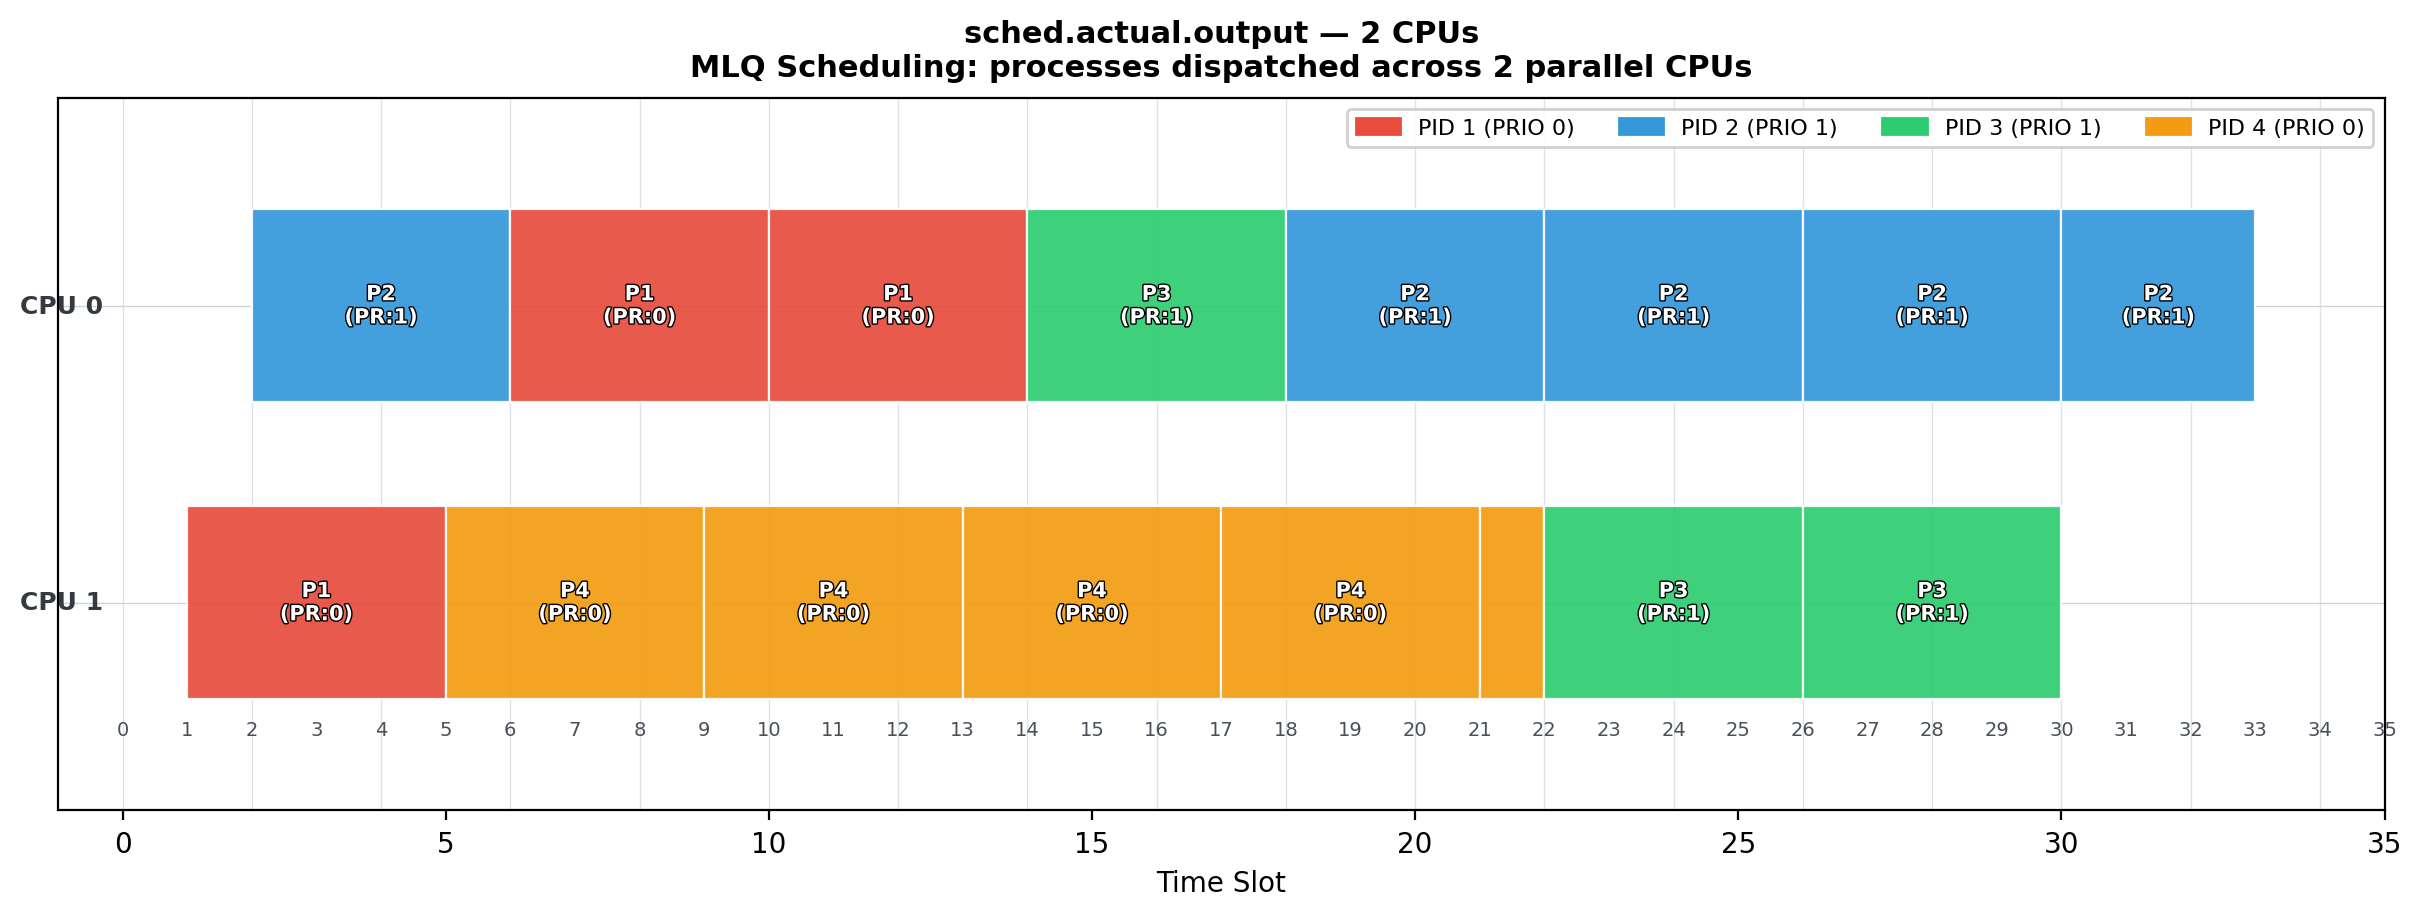
\includegraphics[width=0.8\linewidth]{Images/gantt_sched.png}
    \caption{Gantt Diagram Execution Trace of \texttt{sched.input} (2 CPUs)}
\end{figure}
\begin{figure}[H]
    \centering
    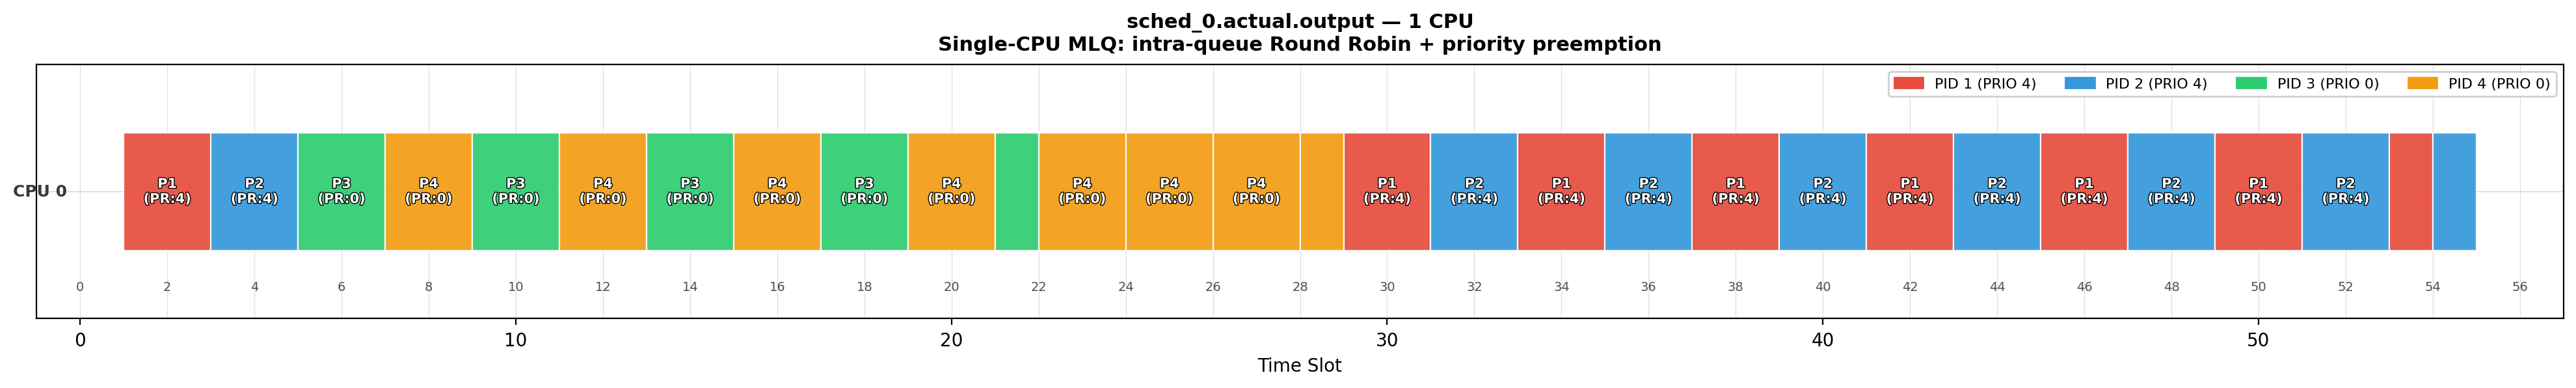
\includegraphics[width=1\linewidth]{Images/gantt_sched_0.png}
    \caption{Gantt Diagram Execution Trace of \texttt{sched\_0.input} (1 CPU)}
\end{figure}
\begin{figure}[H]
    \centering
    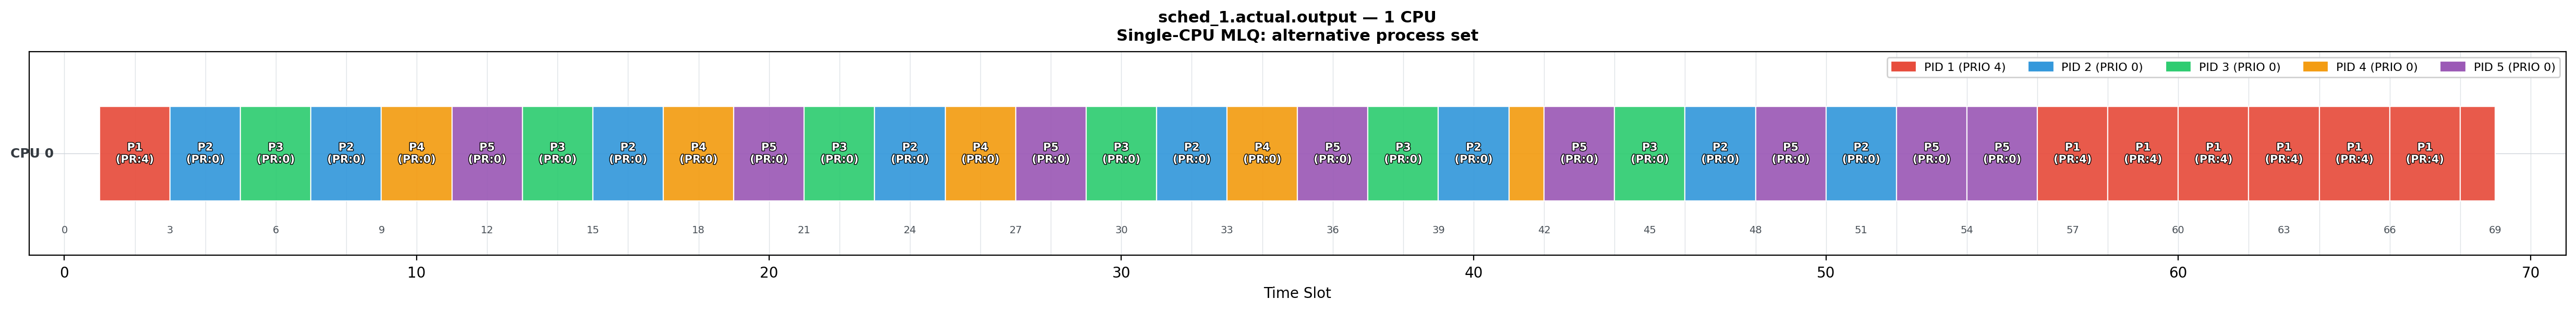
\includegraphics[width=1\linewidth]{Images/gantt_sched_1.png}
    \caption{Gantt Diagram Execution Trace of \texttt{sched\_1.input} (1 CPU)}
\end{figure}
\section{Memory Management}
\subsection{Virtual Memory Architecture}
The memory manager utilizes a paging scheme to separate the physical memory (RAM and SWAP) from the contiguous virtual addresses seen by user processes.

The virtual memory subsystem tracks allocations at three levels:
\begin{enumerate}
    \item \textbf{Virtual Memory Areas (\texttt{vm\_area\_struct}):} Represents large contiguous chunks of virtual memory. Each area maintains a \texttt{sbrk} pointer representing the top of the heap. Memory beneath \texttt{sbrk} is managed by \texttt{vm\_freerg\_list}, which keeps track of freed regions to combat internal fragmentation.
    \item \textbf{Symbol Table (\texttt{symrgtbl}):} Since processes execute simple instructions via registers, this table maps register indices (0 to 29) to allocated virtual memory regions. Each entry is a \texttt{vm\_rg\_struct} with \texttt{rg\_start} and \texttt{rg\_end} fields defining the byte range. The table size is fixed at \texttt{PAGING\_MAX\_SYMTBL\_SZ = 30}.
    \item \textbf{Page Tables:} Translates virtual pages to physical frames. In the 64-bit build (\texttt{MM64}), this is a 5-level hierarchy (PGD $\to$ P4D $\to$ PUD $\to$ PMD $\to$ PT). In the legacy 32-bit build, a single flat \texttt{pgd} array is used.
\end{enumerate}

\subsection{The ALLOC Operation (\texttt{liballoc})}
When a user process issues an \texttt{alloc [size] [reg]} instruction, \texttt{liballoc()} handles it via a highly optimized Two-Phase Allocation Strategy.

\begin{infobox}[Two-Phase Allocation Strategy]
\textbf{Phase 1: Memory Reuse (First-Fit Algorithm)}\\
Before requesting new pages from the kernel, the system scans \texttt{vm\_freerg\_list} via \texttt{get\_free\_vmrg\_area()}. If a previously freed block is large enough, it assigns the block to the requested register, avoiding expensive kernel system calls. The first-fit traversal splits the chosen region: the requested portion is assigned to the symbol table, and any leftover space remains in the free list.

\textbf{Phase 2: Heap Extension (System Call)}\\
If no free blocks are suitable, the system invokes \texttt{SYSMEM\_INC\_OP} via \texttt{\_syscall(caller->krnl, caller->pid, 17, \&regs)} to ask the kernel to increase \texttt{sbrk}. The size is page-aligned using \texttt{PAGING\_PAGE\_ALIGNSZ(size)} (padded to the next multiple of page size). The kernel handler \texttt{inc\_vma\_limit()} expands the VMA boundary, calls \texttt{vm\_map\_ram()} to allocate physical frames and populate page table entries, and advances \texttt{sbrk}. Leftover space from the page-aligned expansion is added back to \texttt{vm\_freerg\_list} for future first-fit allocations.
\end{infobox}

\begin{lstlisting}[language=C, caption=Heap Extension via \texttt{\_syscall} (\texttt{libmem.c})]
int __alloc(struct pcb_t *caller, int vmaid, int rgid, 
            addr_t size, addr_t *alloc_addr)
{
  pthread_mutex_lock(&mmvm_lock);
  struct vm_area_struct *cur_vma = get_vma_by_num(caller->krnl->mm, vmaid);

  // Phase 1: Try to reuse a freed region
  if (get_free_vmrg_area(caller, vmaid, size, &rgnode) == 0) {
    caller->krnl->mm->symrgtbl[rgid].rg_start = rgnode.rg_start;
    caller->krnl->mm->symrgtbl[rgid].rg_end = rgnode.rg_end;
    *alloc_addr = rgnode.rg_start;
    pthread_mutex_unlock(&mmvm_lock);
    return 0;
  }

  // Phase 2: Expand the heap via system call
  int old_sbrk = cur_vma->sbrk;
  struct sc_regs regs;
  regs.a1 = SYSMEM_INC_OP;
  regs.a2 = vmaid;
  regs.a3 = PAGING_PAGE_ALIGNSZ(size);
  _syscall(caller->krnl, caller->pid, 17, &regs);

  // Register the expanded region in the symbol table
  caller->krnl->mm->symrgtbl[rgid].rg_start = old_sbrk;
  caller->krnl->mm->symrgtbl[rgid].rg_end = old_sbrk + size;
  *alloc_addr = old_sbrk;

  pthread_mutex_unlock(&mmvm_lock);
  return 0;
}
\end{lstlisting}

\subsection{The FREE Operation (\texttt{\_\_free})}
The \texttt{free [reg]} instruction is non-destructive to the physical page table.
\begin{lstlisting}[language=C, caption=FREE implementation (\texttt{libmem.c})]
int __free(struct pcb_t *caller, int vmaid, int rgid) {
    pthread_mutex_lock(&mmvm_lock);
    struct vm_rg_struct *rgnode = get_symrg_byid(caller->krnl->mm, rgid);
    
    if (rgnode->rg_start == 0 && rgnode->rg_end == 0) {
        pthread_mutex_unlock(&mmvm_lock);
        return -1; // Nothing to free (never allocated)
    }
    
    // Copy the region to a new free node
    struct vm_rg_struct *freerg_node = malloc(sizeof(struct vm_rg_struct));
    freerg_node->rg_start = rgnode->rg_start;
    freerg_node->rg_end = rgnode->rg_end;
    freerg_node->rg_next = NULL;

    // Erase from symbol table and add to free list
    rgnode->rg_start = rgnode->rg_end = 0;
    rgnode->rg_next = NULL;
    enlist_vm_freerg_list(caller->krnl->mm, freerg_node);
    pthread_mutex_unlock(&mmvm_lock);
    return 0;
}
\end{lstlisting}
\textbf{Analysis:} By choosing not to deallocate the physical frames immediately, the OS significantly reduces the overhead of page table manipulation. Re-allocating the same space later instantly succeeds via Phase 1. Note the guard check \texttt{rg\_start == 0 \&\& rg\_end == 0}: if a register was never allocated (e.g., a blocked \texttt{KMALLOC} instruction), the free operation returns $-1$. This produces the \texttt{libfree:218 failed} message seen in the execution traces.

\subsection{READ/WRITE \& Page Replacement Strategy}
Reads and Writes are handled by \texttt{\_\_read} and \texttt{\_\_write}. These traverse the virtual bounds to find the exact byte.

\begin{lstlisting}[language=C, caption=Reading Virtual Memory (\texttt{libmem.c})]
int pg_getval(struct mm_struct *mm, int addr, BYTE *data, struct pcb_t *caller) {
    int pgn = PAGING_PGN(addr);
    int off = PAGING_OFFST(addr);
    int fpn;

    /* Get the page to RAM. Handles page faults internally! */
    if (pg_getpage(mm, pgn, &fpn, caller) != 0) 
        return -1;

    int phyaddr = (fpn << PAGING_ADDR_FPN_LOBIT) + off;
    
    struct sc_regs regs;
    regs.a1 = SYSMEM_IO_READ;
    regs.a2 = phyaddr;
    regs.a3 = 0;
    _syscall(caller->krnl, caller->pid, 17, &regs);
    *data = (BYTE)regs.a3;
    return 0;
}
\end{lstlisting}

\begin{theorybox}[Physical Address Computation]
The physical address is computed as \texttt{(fpn << PAGING\_ADDR\_FPN\_LOBIT) + off}, which is equivalent to \texttt{fpn * PAGING\_PAGESZ + off}. The bit-shift formulation is used because \texttt{PAGING\_ADDR\_FPN\_LOBIT} equals $\log_2(\texttt{PAGING\_PAGESZ})$, and left-shifting by this value is a faster equivalent of multiplication by the page size. The read/write operations themselves are performed through the system call interface (\texttt{SYSMEM\_IO\_READ}/\texttt{SYSMEM\_IO\_WRITE}) to maintain the user--kernel boundary: the actual \texttt{MEMPHY\_read}/\texttt{MEMPHY\_write} calls happen inside \texttt{\_\_sys\_memmap} in kernel space.
\end{theorybox}

\subsection{Detailed Page Fault Mechanics}
If the page resides in SWAP instead of RAM, \texttt{pg\_getpage()} triggers a \textbf{Page Fault}. The kernel intercepts this and initiates a Page Replacement sequence using a strict FIFO queue (\texttt{mm->fifo\_pgn}):

\textbf{Case 1: Free frame available.} If \texttt{MEMPHY\_get\_freefp()} succeeds, the page is assigned the free frame directly via \texttt{pte\_set\_fpn()} and added to the FIFO list.

\textbf{Case 2: No free frames (full replacement path):}
\begin{enumerate}
    \item \textbf{Find Victim:} Dequeue the oldest page from \texttt{fifo\_pgn} using \texttt{find\_victim\_page()}. This function walks the singly-linked list to find the \textbf{tail node}---the oldest entry---implementing true FIFO ordering.
    \item \textbf{Swap Out:} Copy the victim page from RAM into the secondary SWAP device using \texttt{\_\_swap\_cp\_page(mram, vicfpn, active\_mswp, swpfpn)}. Update the victim's PTE via \texttt{pte\_set\_swap()} to record the swap device ID and swap offset.
    \item \textbf{Swap In:} If the requested page was previously swapped out (indicated by the \texttt{PAGING\_PTE\_SWAPPED\_MASK} bit), copy it back from SWAP to the victim's freed frame. Otherwise, zero-fill the frame (new allocation).
    \item \textbf{Update PTEs:} Update the Page Table Entry for the newly loaded page via \texttt{pte\_set\_fpn()} to clear the swapped bit and set the FPN. Push the newly loaded page into \texttt{fifo\_pgn}.
\end{enumerate}

\textbf{Example of a Page Fault:}\\
Assume RAM has exactly 2 frames. Process 1 requests 3 pages.
1. CPU executes \texttt{alloc 512} (Page 0 and Page 1). RAM Frame 0 and 1 are used.
2. CPU executes alloc 256 (Page 2). RAM is full. The OS triggers a Page Replacement (Swapping) sequence.3. The OS selects Page 0 (oldest) as the victim. 
4. \texttt{\_\_swap\_cp\_page(RAM, 0, SWAP, 0)} is called. Page 0 is now on disk.
5. RAM Frame 0 is now assigned to Page 2. 
6. If the CPU subsequently tries to read Page 0, a \textit{second} Page Fault occurs. The OS will select Page 1 as the victim, swap it to disk, and bring Page 0 back into RAM Frame 1.

\subsection{Kernel Memory Operations}
The specification defines three kernel-space memory instructions that enable privileged allocation patterns modeled after Linux's kernel memory subsystem. These are implemented in \texttt{libmem.c} and protected by the \texttt{mode\_bit} check described in Section 2.

\subsubsection{\texttt{KMALLOC} --- Physically Contiguous Allocation}
The \texttt{kmalloc [size] [reg]} instruction allocates a contiguous block of \textit{physical} memory. Unlike user-space \texttt{ALLOC} which allows the OS to scatter pages across non-contiguous frames, \texttt{KMALLOC} requires that the allocated frames form a \textbf{consecutive sequence} in physical RAM:
\begin{lstlisting}[language=C, caption=\texttt{\_\_kmalloc} contiguity check (\texttt{libmem.c})]
addr_t __kmalloc(struct pcb_t *caller, int vmaid, int rgid, 
                 addr_t size, addr_t *alloc_addr)
{
  // First, attempt a normal virtual allocation
  if (__alloc(caller, 0, rgid, size, alloc_addr) < 0)
    return (addr_t)-1;

  // Then verify physical contiguity
  if (!is_phys_contiguous_region(caller, *alloc_addr, size)) {
    __free(caller, 0, rgid); // Roll back
    return (addr_t)-1;
  }
  return *alloc_addr;
}
\end{lstlisting}
The helper \texttt{is\_phys\_contiguous\_region()} walks the page table entries for the allocated virtual range and verifies that each successive PTE's frame page number (FPN) is exactly one greater than the previous. If the frames are scattered, the allocation is rolled back. This models real-world DMA buffers and kernel data structures that require contiguous physical memory.

\subsubsection{User/Kernel Address Tagging}
To distinguish user-space allocations from kernel-space allocations, the system uses a \textbf{tag bit} mechanism:
\begin{lstlisting}[language=C, caption=Address tagging (\texttt{libmem.c})]
#ifdef MM64
#define KERNEL_ADDR_TAG ((addr_t)1ULL << 63)
#else
#define KERNEL_ADDR_TAG ((addr_t)1U << 31)
#endif

static int is_kernel_addr(addr_t addr) {
  return (addr & KERNEL_ADDR_TAG) != 0;
}
static addr_t to_kernel_addr(addr_t addr) {
  return addr | KERNEL_ADDR_TAG;
}
\end{lstlisting}
When \texttt{libkmem\_malloc()} stores a kernel allocation address in a register, it tags the address by setting the most-significant bit (bit 63 for 64-bit, bit 31 for 32-bit): \texttt{caller->regs[reg\_index] = to\_kernel\_addr(addr)}. Subsequent \texttt{libread}/\texttt{libwrite} calls check \texttt{is\_kernel\_addr()} and \textbf{reject} user-mode accesses to kernel-tagged addresses. This mirrors the canonical address split in real x86-64 architectures, where user-space addresses have their top bits clear and kernel-space addresses have them set.

\subsubsection{Slab Cache: \texttt{KMEM\_CACHE\_CREATE} \& \texttt{KMEM\_CACHE\_ALLOC}}
The slab allocator avoids repeated allocation/initialization overhead by pre-defining fixed-size object pools:
\begin{lstlisting}[language=C, caption=Cache pool creation (\texttt{libmem.c})]
int libkmem_cache_pool_create(struct pcb_t *caller, uint32_t size, 
                              uint32_t align, uint32_t cache_pool_id)
{
  if (caller->krnl->mm->kcpooltbl == NULL)
    caller->krnl->mm->kcpooltbl = calloc(PAGING_MAX_SYMTBL_SZ, 
                                          sizeof(struct kcache_pool_struct));

  if (cache_pool_id >= PAGING_MAX_SYMTBL_SZ)
    return -1;

  caller->krnl->mm->kcpooltbl[cache_pool_id].size = size;
  caller->krnl->mm->kcpooltbl[cache_pool_id].align = align;
  caller->krnl->mm->kcpooltbl[cache_pool_id].storage = 0;
  return 0;
}
\end{lstlisting}
\texttt{KMEM\_CACHE\_CREATE} registers a cache pool with a predefined object size and alignment. When \texttt{KMEM\_CACHE\_ALLOC} is later called, it delegates to \texttt{\_\_kmalloc} using the pool's stored size, guaranteeing that every allocation from the same cache pool produces physically contiguous blocks of identical size. This mirrors the Linux kernel's \texttt{kmem\_cache\_create()}/\texttt{kmem\_cache\_alloc()} API.

\subsubsection{\texttt{COPY\_FROM\_USER} \& \texttt{COPY\_TO\_USER}}
These instructions enable safe data transfer across the user/kernel boundary:
\begin{lstlisting}[language=C, caption=Cross-boundary memory copy (\texttt{libmem.c})]
int libkmem_copy_from_user(struct pcb_t *caller, uint32_t source, 
                           uint32_t destination, uint32_t offset, 
                           uint32_t size) {
  uint32_t i;
  BYTE data;
  for (i = 0; i < size; i++) {
    if (__read_user_mem(caller, 0, source, offset + i, &data) < 0)
      return -1;
    if (__write_kernel_mem(caller, 0, destination, i, data) < 0)
      return -1;
  }
  return 0;
}
\end{lstlisting}
\texttt{COPY\_FROM\_USER} reads byte-by-byte from a user-space region and writes to a kernel-space region. \texttt{COPY\_TO\_USER} performs the reverse. The helper functions \texttt{\_\_read\_user\_mem} and \texttt{\_\_write\_kernel\_mem} enforce address-space isolation: \texttt{\_\_read\_user\_mem} rejects reads from kernel-tagged addresses (via \texttt{is\_kernel\_addr()}), and \texttt{\_\_write\_kernel\_mem} rejects writes to non-kernel-tagged addresses. This prevents user processes from smuggling kernel pointers to escalate privileges.
\section{System Call Integration}
A robust OS must isolate kernel memory from user processes. The \texttt{memmap} interface (Syscall number 17, dispatched via \texttt{libsyscall}) guarantees this protection.

\begin{infobox}[Terminology Clarification: Opcode vs. Syscall Number]
In this simulator, \texttt{SYSCALL} is an \textbf{instruction opcode} (defined in \texttt{common.h}'s \texttt{enum ins\_opcode\_t}). When \texttt{cpu.c:run()} encounters this opcode, it calls \texttt{libsyscall(proc, arg\_0, arg\_1, arg\_2, arg\_3)} and sandwiches the call between \texttt{mode\_bit = 0} (Kernel) and \texttt{mode\_bit = 1} (User) transitions. Inside \texttt{libsyscall}, argument \texttt{arg\_0} carries the \textbf{syscall number} (e.g., 17 for \texttt{\_\_sys\_memmap}), which is then dispatched through \texttt{syscalltbl.lst}. The two concepts --- the opcode \texttt{SYSCALL} and the syscall number 17 --- are distinct.
\end{infobox}

\subsection{Register-Based Argument Passing}
Arguments are packed into a \texttt{sc\_regs} structure. Register \texttt{a1} contains the operation code, while \texttt{a2} and \texttt{a3} hold arguments.

\vspace{0.5em}
\begin{table}[H]
    \centering
    \renewcommand{\arraystretch}{1.2}
    \begin{tabular}{|l|p{8cm}|}
    \hline
    \textbf{Opcode} & \textbf{Kernel Action} \\
    \hline
    \texttt{SYSMEM\_MAP\_OP (1)} & Executes \texttt{vmap\_pgd\_memset()} to emulate page directory behavior. \\
    \texttt{SYSMEM\_INC\_OP (2)} & Executes \texttt{inc\_vma\_limit()} to safely expand the heap. \\
    \texttt{SYSMEM\_SWP\_OP (3)} & Executes \texttt{\_\_mm\_swap\_page()} for disk swapping. \\
    \texttt{SYSMEM\_IO\_READ (4)} & Reads exactly 1 byte from physical memory. \\
    \texttt{SYSMEM\_IO\_WRITE (5)} & Writes exactly 1 byte to physical memory. \\
    \hline
    \end{tabular}
    \caption{SYSCALL 17 Operations}
\end{table}
\vspace{0.5em}

\subsection{System Call Dispatching and Protection}
The kernel provides a centralized dispatcher that validates every request. The function \texttt{\_syscall()} (with a leading underscore, defined in \texttt{syscall.c}) uses C preprocessor X-macros to dynamically build its dispatch switch statement from the \texttt{syscalltbl.lst} file:

\vspace{0.5em}
\begin{lstlisting}[language=C, caption=Kernel Syscall Dispatcher (\texttt{syscall.c})]
#define __SYSCALL(nr, sym) case nr: return __##sym(krnl,pid,regs);
int _syscall(struct krnl_t *krnl, uint32_t pid, uint32_t nr, 
             struct sc_regs* regs)
{
    switch (nr) {
    #include "syscalltbl.lst"
    default: return __sys_ni_syscall(krnl, regs);
    }
};

// syscalltbl.lst contains:
// __SYSCALL(0, sys_listsyscall)
// __SYSCALL(17, sys_memmap)
\end{lstlisting}
\vspace{0.5em}
The X-macro \texttt{\_\_SYSCALL(nr, sym)} expands each line of \texttt{syscalltbl.lst} into a \texttt{case} statement. For example, \texttt{\_\_SYSCALL(17, sys\_memmap)} becomes \texttt{case 17: return \_\_sys\_memmap(krnl, pid, regs);}.  The \texttt{\_\_sys\_ni\_syscall} default handler safely ignores invalid syscall numbers.

\subsection{PID-Based Kernel Traversal}
The specification explicitly requires: ``\textit{The process PCB is prohibited from being passed directly. It must be accessed by traversing in kernel mode to obtain the PCB from the kernel structure using the given PID.}'' The system call handler \texttt{\_\_sys\_memmap()} in \texttt{sys\_mem.c} adheres to this requirement:

\begin{lstlisting}[language=C, caption=PID-based process lookup in \texttt{\_\_sys\_memmap} (\texttt{sys\_mem.c})]
int __sys_memmap(struct krnl_t *krnl, uint32_t pid, struct sc_regs* regs) {
    int memop = regs->a1;
    BYTE value;
    
    /* Resolve caller by PID -- NOT by passing pcb_t* directly */
    struct pcb_t *caller = find_proc_by_pid(pid);
    if (caller == NULL) return -1;
    
    switch (memop) {
    case SYSMEM_MAP_OP:  vmap_pgd_memset(caller, regs->a2, regs->a3); break;
    case SYSMEM_INC_OP:  inc_vma_limit(caller, regs->a2, regs->a3); break;
    case SYSMEM_SWP_OP:  __mm_swap_page(caller, regs->a2, regs->a3); break;
    case SYSMEM_IO_READ:
        MEMPHY_read(krnl->mram, regs->a2, &value);
        regs->a3 = value;
        break;
    case SYSMEM_IO_WRITE:
        MEMPHY_write(krnl->mram, regs->a2, regs->a3);
        break;
    }
    return 0;
}
\end{lstlisting}

The \texttt{find\_proc\_by\_pid()} function (in \texttt{sched.c}) traverses two data structures under the global \texttt{queue\_lock} mutex:
\begin{enumerate}
    \item \textbf{The \texttt{running\_list}:} Searched first, since the caller is most likely currently running.
    \item \textbf{All 140 MLQ ready queues:} Searched sequentially if the process is not found in the running list (possible during concurrent scheduling transitions).
\end{enumerate}
This PID-based lookup ensures that the system call handler operates entirely in kernel space, using only the PID as a numeric handle. The user process never passes its \texttt{pcb\_t*} pointer across the user/kernel boundary, preventing forged pointer attacks.

\subsection{Wrapper Library (\texttt{libstd.c})}
The user-space library \texttt{libsyscall()} in \texttt{libstd.c} acts as a thin wrapper that packs arguments into a \texttt{sc\_regs} structure and invokes the kernel dispatcher:
\begin{lstlisting}[language=C, caption=User-space syscall wrapper (\texttt{libstd.c})]
int libsyscall(struct pcb_t *caller,
               uint32_t syscall_idx,
               arg_t a1, arg_t a2, arg_t a3)
{
   struct sc_regs regs;
   regs.a1 = a1;
   regs.a2 = a2;
   regs.a3 = a3;
   return _syscall(caller->krnl, caller->pid, syscall_idx, &regs);
}
\end{lstlisting}

\noindent\textbf{Protection and Isolation:} Without system calls, a process could manually manipulate its \texttt{struct pcb\_t} and page tables to read another user's data or crash the system. By forcing the user to call \texttt{syscall(17)}, the CPU switches to Kernel Mode and resolves the caller by PID. The \texttt{SYSMEM\_IO\_READ} and \texttt{SYSMEM\_IO\_WRITE} operations access physical memory through \texttt{krnl->mram}---the kernel's own memory reference---rather than any user-provided pointer. Argument validation and alignment handling are then enforced in downstream memory-management routines (for example, \texttt{inc\_vma\_limit()} and related VM helpers).
\section{Multi-level Paging (64-bit Scheme)}
To handle the massive 128 PiB virtual address space associated with a 64-bit architecture, the standard single-level page table is highly inefficient. We implemented a 5-level page table scheme in \texttt{mm64.c}.

\subsection{Address Translation Process}
The 64-bit virtual address is segmented using strict bitmasks:
\begin{lstlisting}[language=C, caption=5-Level Address Bit Extraction (\texttt{mm64.c})]
int get_pd_from_address(addr_t addr, addr_t* pgd, addr_t* p4d, addr_t* pud, addr_t* pmd, addr_t* pt) {
    *pgd = (addr & PAGING64_ADDR_PGD_MASK) >> PAGING64_ADDR_PGD_LOBIT; // bits 48-56
    *p4d = (addr & PAGING64_ADDR_P4D_MASK) >> PAGING64_ADDR_P4D_LOBIT; // bits 39-47
    *pud = (addr & PAGING64_ADDR_PUD_MASK) >> PAGING64_ADDR_PUD_LOBIT; // bits 30-38
    *pmd = (addr & PAGING64_ADDR_PMD_MASK) >> PAGING64_ADDR_PMD_LOBIT; // bits 21-29
    *pt  = (addr & PAGING64_ADDR_PT_MASK)  >> PAGING64_ADDR_PT_LOBIT;  // bits 12-20

    if (((addr >> PAGING64_ADDR_PGD_HIBIT) & 0x1) != 0) {
        /* Kernel-space canonical address: high bits must stay 1 */
        *pgd |= BIT_ULL(PAGING64_ADDR_PGD_HIBIT - PAGING64_ADDR_PGD_LOBIT);
    }
    return 0;
}
\end{lstlisting}

Given a user-space virtual address of 0x0000000000400000 (4MB), the extraction process yields the following indices: 

\begin{itemize}
    \item \textbf{PGD Index:} $(0\text{x}400000 \gg 48) \ \& \ 0\text{x}1\text{FF} = 0$
    \item \textbf{P4D Index:} $(0\text{x}400000 \gg 39) \ \& \ 0\text{x}1\text{FF} = 0$
    \item \textbf{PUD Index:} $(0\text{x}400000 \gg 30) \ \& \ 0\text{x}1\text{FF} = 0$
    \item \textbf{PMD Index:} $(0\text{x}400000 \gg 21) \ \& \ 0\text{x}1\text{FF} = 2$
    \item \textbf{PT Index:} $(0\text{x}400000 \gg 12) \ \& \ 0\text{x}1\text{FF} = 0$
\end{itemize}

The virtual address \texttt{0x0000000000400000} is translated through

\[
\mathrm{PGD}[0] \rightarrow \mathrm{P4D}[0] \rightarrow \mathrm{PUD}[0]
\rightarrow \mathrm{PMD}[2] \rightarrow \mathrm{PT}[0]
\] 

\subsection{Canonical Address Handling}
In a 64-bit architecture, the hardware typically implements only 48-bit or 57-bit addressing rather than the full 64-bit range. To prevent software from misusing the unused higher-order bits for non-address purposes, the architecture enforces \textbf{canonical addresses}: all unused bits must be copies of the highest implemented bit (sign-extension).

In our implementation, \texttt{get\_pd\_from\_address()} checks bit 56 (the \texttt{PAGING64\_ADDR\_PGD\_HIBIT}). If this bit is set, the address belongs to \textbf{kernel space}, and the PGD index is OR-ed with an extra high bit to push it into the upper half of the PGD array. This creates a clean split:
\begin{itemize}
    \item \textbf{User-space addresses} (bits 63--57 all zero): PGD indices $0$ to $\sim255$
    \item \textbf{Kernel-space addresses} (bits 63--57 all ones): PGD indices $256+$
\end{itemize}
This mirrors Linux's 5-level paging layout where the canonical address hole between \texttt{0x00ffffffffffffff} and \texttt{0xff00000000000000} is unmappable, ensuring user processes cannot access kernel memory through arithmetic overflow.

\subsection{PTE Bit Layout}
Each Page Table Entry (PTE) stores essential metadata, defined by bitmask macros in \texttt{mm64.h}:
\begin{itemize}
    \item \textbf{Present bit (\texttt{PAGING\_PTE\_PRESENT\_MASK}):} Set to 1 if the page is in RAM; 0 means a page fault is required on access.
    \item \textbf{Swapped bit (\texttt{PAGING\_PTE\_SWAPPED\_MASK}):} Set to 1 if the page data currently resides on the SWAP device.
    \item \textbf{Dirty bit (\texttt{PAGING\_PTE\_DIRTY\_MASK}):} Set to 1 if the page has been written since it was last loaded from swap.
    \item \textbf{Frame Page Number (\texttt{PAGING\_PTE\_FPN\_MASK}, low bits):} The actual Physical Frame Number assigned to this virtual page.
    \item \textbf{Swap type/offset (\texttt{PAGING\_PTE\_SWPTYP\_MASK} / \texttt{PAGING\_PTE\_SWPOFF\_MASK}):} When the page is swapped out, these fields record which swap device and at which offset the page data resides.
\end{itemize}

\subsection{Hierarchical Entry Population}
\begin{lstlisting}[language=C, caption=Setting a PTE with 5-level hierarchy (\texttt{mm64.c})]
int pte_set_fpn(struct pcb_t *caller, addr_t pgn, addr_t fpn) {
    addr_t pgd=0, p4d=0, pud=0, pmd=0, pt=0;
    struct krnl_t *krnl = caller->krnl;

    get_pd_from_pagenum(pgn, &pgd, &p4d, &pud, &pmd, &pt);
    
    /* Set intermediate directory entries as present */
    init_pte(&krnl->mm->pgd[pgd % PAGING64_MAX_PGN], 1, p4d + 1, 0, 0, 0, 0);
    init_pte(&krnl->mm->p4d[p4d % PAGING64_MAX_PGN], 1, pud + 1, 0, 0, 0, 0);
    init_pte(&krnl->mm->pud[pud % PAGING64_MAX_PGN], 1, pmd + 1, 0, 0, 0, 0);
    init_pte(&krnl->mm->pmd[pmd % PAGING64_MAX_PGN], 1, pt + 1, 0, 0, 0, 0);
    
    addr_t *pte = &krnl->mm->pt[pgn % PAGING64_MAX_PGN];

    SETBIT(*pte, PAGING_PTE_PRESENT_MASK);
    CLRBIT(*pte, PAGING_PTE_SWAPPED_MASK);
    SETVAL(*pte, fpn, PAGING_PTE_FPN_MASK, PAGING_PTE_FPN_LOBIT);
    return 0;
}
\end{lstlisting}

\begin{theorybox}[Design Decision: Pre-Allocated vs. Sparse Page Tables]
\textbf{Production operating systems} such as Linux implement true sparse hierarchical page tables: lower-level directories (P4D, PUD, PMD, PT) are allocated on demand via \texttt{get\_free\_page()} only when a virtual address in that range is first accessed. This means a process using only 1 MB of heap allocates a tiny fraction of the theoretical page table space.

\textbf{Our simulator} adopts a different trade-off. In \texttt{init\_mm()} (\texttt{mm64.c:447--451}), all five paging-level arrays are \textbf{pre-allocated as fixed-size flat arrays} using \texttt{calloc(PAGING64\_MAX\_PGN, sizeof(addr\_t))}:
\begin{lstlisting}[language=C]
mm->pgd = calloc(PAGING64_MAX_PGN, sizeof(addr_t));
mm->p4d = calloc(PAGING64_MAX_PGN, sizeof(addr_t));
mm->pud = calloc(PAGING64_MAX_PGN, sizeof(addr_t));
mm->pmd = calloc(PAGING64_MAX_PGN, sizeof(addr_t));
mm->pt  = calloc(PAGING64_MAX_PGN, sizeof(addr_t));
\end{lstlisting}
This sacrifices memory efficiency in favor of simplicity and direct array-based indexing (\texttt{O(1)} access via modular arithmetic). The \texttt{pte\_set\_fpn} function still populates the hierarchy chain \textit{logically} by marking PGD$\to$P4D$\to$PUD$\to$PMD entries as present only when pages are mapped, demonstrating the correctness of the multi-level translation mechanism.
\end{theorybox}

\subsection{The \texttt{vmap\_pgd\_memset} System Call}
The specification requires students to implement a \texttt{vmap\_pgd\_memset} operation to emulate page directory behavior for the 64-bit address scheme. This operation is invoked through \texttt{SYSMEM\_MAP\_OP} (syscall 17, operation code 1):
\begin{lstlisting}[language=C, caption=\texttt{vmap\_pgd\_memset} (\texttt{mm64.c})]
int vmap_pgd_memset(struct pcb_t *caller, addr_t addr, int pgnum) {
    int pgit;
    addr_t pgn = (addr >> PAGING64_ADDR_PT_SHIFT);
    addr_t pattern = 0xdeadbeefUL;

    for (pgit = 0; pgit < pgnum; pgit++) {
        caller->krnl->mm->pt[(pgn + pgit) % PAGING64_MAX_PGN] = pattern;
    }
    return 0;
}
\end{lstlisting}
This function fills \texttt{pgnum} consecutive page table entries with the sentinel pattern \texttt{0xdeadbeef}. This serves as a dummy allocation used to test and verify that the 64-bit address scheme's page directory traversal is functioning correctly without performing real physical memory allocation.

\subsection{Quantitative Statistics (Required by Specification)}
The specification asks for statistics on memory access activity and multi-level paging storage size. We report both here.

\textbf{1) Multi-level paging storage size}\\
From \texttt{mm64.h},
\[
\texttt{PAGING64\_MAX\_PGN} = \left\lceil \frac{2^{21}}{4096} \right\rceil = 512
\]
Each paging level array stores 512 entries of type \texttt{addr\_t} (8 bytes on 64-bit):
\[
512 \times 8 = 4096\ \text{bytes per level}
\]
With 5 levels (PGD, P4D, PUD, PMD, PT):
\[
5 \times 4096 = 20480\ \text{bytes} = 20\ \text{KiB per process mm}
\]
This matches the \texttt{calloc(PAGING64\_MAX\_PGN, sizeof(addr\_t))} allocation pattern in \texttt{init\_mm()}.

\textbf{2) Memory access activity statistics from actual outputs}\\
We use trace-observable memory-management events (allocation/free logs and page-table dumps) from provided outputs:

\begin{table}[!htbp]
\centering
\small
\renewcommand{\arraystretch}{1.2}
\begin{tabularx}{\linewidth}{|>{\ttfamily\footnotesize\raggedright\arraybackslash}p{0.43\linewidth}|>{\centering\arraybackslash}p{0.10\linewidth}|>{\centering\arraybackslash}p{0.10\linewidth}|>{\centering\arraybackslash}p{0.18\linewidth}|>{\centering\arraybackslash}p{0.11\linewidth}|}
\hline
\textbf{Output file} & \textbf{\texttt{alloc}} & \textbf{\texttt{free}} & \textbf{\texttt{free failed}} & \textbf{\texttt{pgtbl}} \\
\hline
\texttt{os\_1\_mlq\_paging.actual.output} & 9 & 6 & 0 & 23 \\
\hline
\texttt{os\_2\_mlq\_paging.actual.output} & 4 & 4 & 4 & 12 \\
\hline
\end{tabularx}
\caption{Trace-derived memory activity statistics from provided testcase outputs.}
\end{table}

\textbf{3) Translation memory-access cost (analytical)}\\
For 5-level paging without TLB hit, a data access requires up to 5 page-walk reads plus 1 data memory access:
\[
A_{\text{no TLB}} = 5 + 1 = 6
\]
On a TLB hit, only the final data access is required:
\[
A_{\text{TLB hit}} = 1
\]
These figures explain why hierarchical paging is scalable in address-space size but still benefits strongly from TLB locality.
\section{Questionnaire \& Practical Examples}

\begin{questionbox}[Question 1]
\textit{What are the advantages and disadvantages of using the unified system call interface for manipulating different system components (read/write/free for files, memory, and I/O devices)? Consider how this abstraction influences OS design, performance trade-offs, error handling complexity, and the balance between portability and efficiency.}
\end{questionbox}

\textbf{Answer:}\\
The Unix philosophy of \textit{``everything is a file''} abstracts all I/O resources (disks, sockets, pipes, terminals, memory-mapped devices) into a uniform \texttt{file descriptor} handle. Every resource is manipulated via a small set of system calls: \texttt{open()}, \texttt{read()}, \texttt{write()}, \texttt{close()}.

\textbf{Internal Architecture (VFS Layer):}\\
The kernel implements this via the \textbf{Virtual File System (VFS)}, a software indirection layer that maps each syscall to a driver-specific handler through a table of function pointers (\texttt{struct file\_operations}). When a user calls \texttt{write(fd, buf, n)}, the VFS dispatches to the correct handler---whether that is a hard disk driver, a network socket, or a GPU device---without the user knowing which:
\begin{lstlisting}[language=C]
struct file_operations {
    ssize_t (*read)(struct file *, char __user *, size_t, loff_t *);
    ssize_t (*write)(struct file *, const char __user *, size_t, loff_t *);
    int     (*open)(struct inode *, struct file *);
    int     (*release)(struct inode *, struct file *);
};
\end{lstlisting}

\begin{itemize}
    \item \textbf{Advantages:}
    \begin{itemize}
        \item \textit{Portability \& Composability:} A utility like \texttt{cat} that reads \texttt{stdin} works identically whether stdin is a file, a pipe, or a network socket. No code changes are needed.
        \item \textit{Unified Security Model:} POSIX permission bits (\texttt{rwxr-xr-x}) and \texttt{DAC/MAC} policies apply uniformly to all resources through a single mechanism.
        \item \textit{Simplified OS Design:} The kernel only needs one generic buffer-cache subsystem, one locking strategy, and one error-propagation pathway to cover all device types.
        \item \textit{In our OS:} The instruction dispatcher in \texttt{cpu.c} handles \texttt{READ}/\texttt{WRITE}/\texttt{FREE} opcodes directly, while the \texttt{SYSCALL} opcode transitions to kernel mode and routes through \texttt{libsyscall()} and \texttt{\_syscall()} (syscall table in \texttt{syscall.c}). The unification point is therefore the syscall layer, not a per-opcode table in \texttt{cpu.c}.
    \end{itemize}
    \item \textbf{Disadvantages:}
    \begin{itemize}
        \item \textit{Performance Overhead:} Every access passes through VFS indirection layers. A direct memory-mapped I/O (\texttt{mmap}) bypasses this cost entirely, which is why high-performance databases (e.g., PostgreSQL) prefer \texttt{mmap} over \texttt{read()}.
        \item \textit{Imperfect Abstractions:} Network devices require connection state, asynchronous events, and specialized options that cannot fit cleanly into \texttt{read}/\texttt{write}. This forces the use of \texttt{ioctl()} --- an escape hatch that is opaque, non-portable, and notoriously hard to use correctly.
        \item \textit{Error Handling Complexity:} A single \texttt{write()} return value of \texttt{-1} must cover disk-full, network-reset, permission-denied, and hardware-fault conditions. Distinguishing these via \texttt{errno} alone is brittle.
    \end{itemize}
\end{itemize}

\begin{figure}[H]
    \centering
    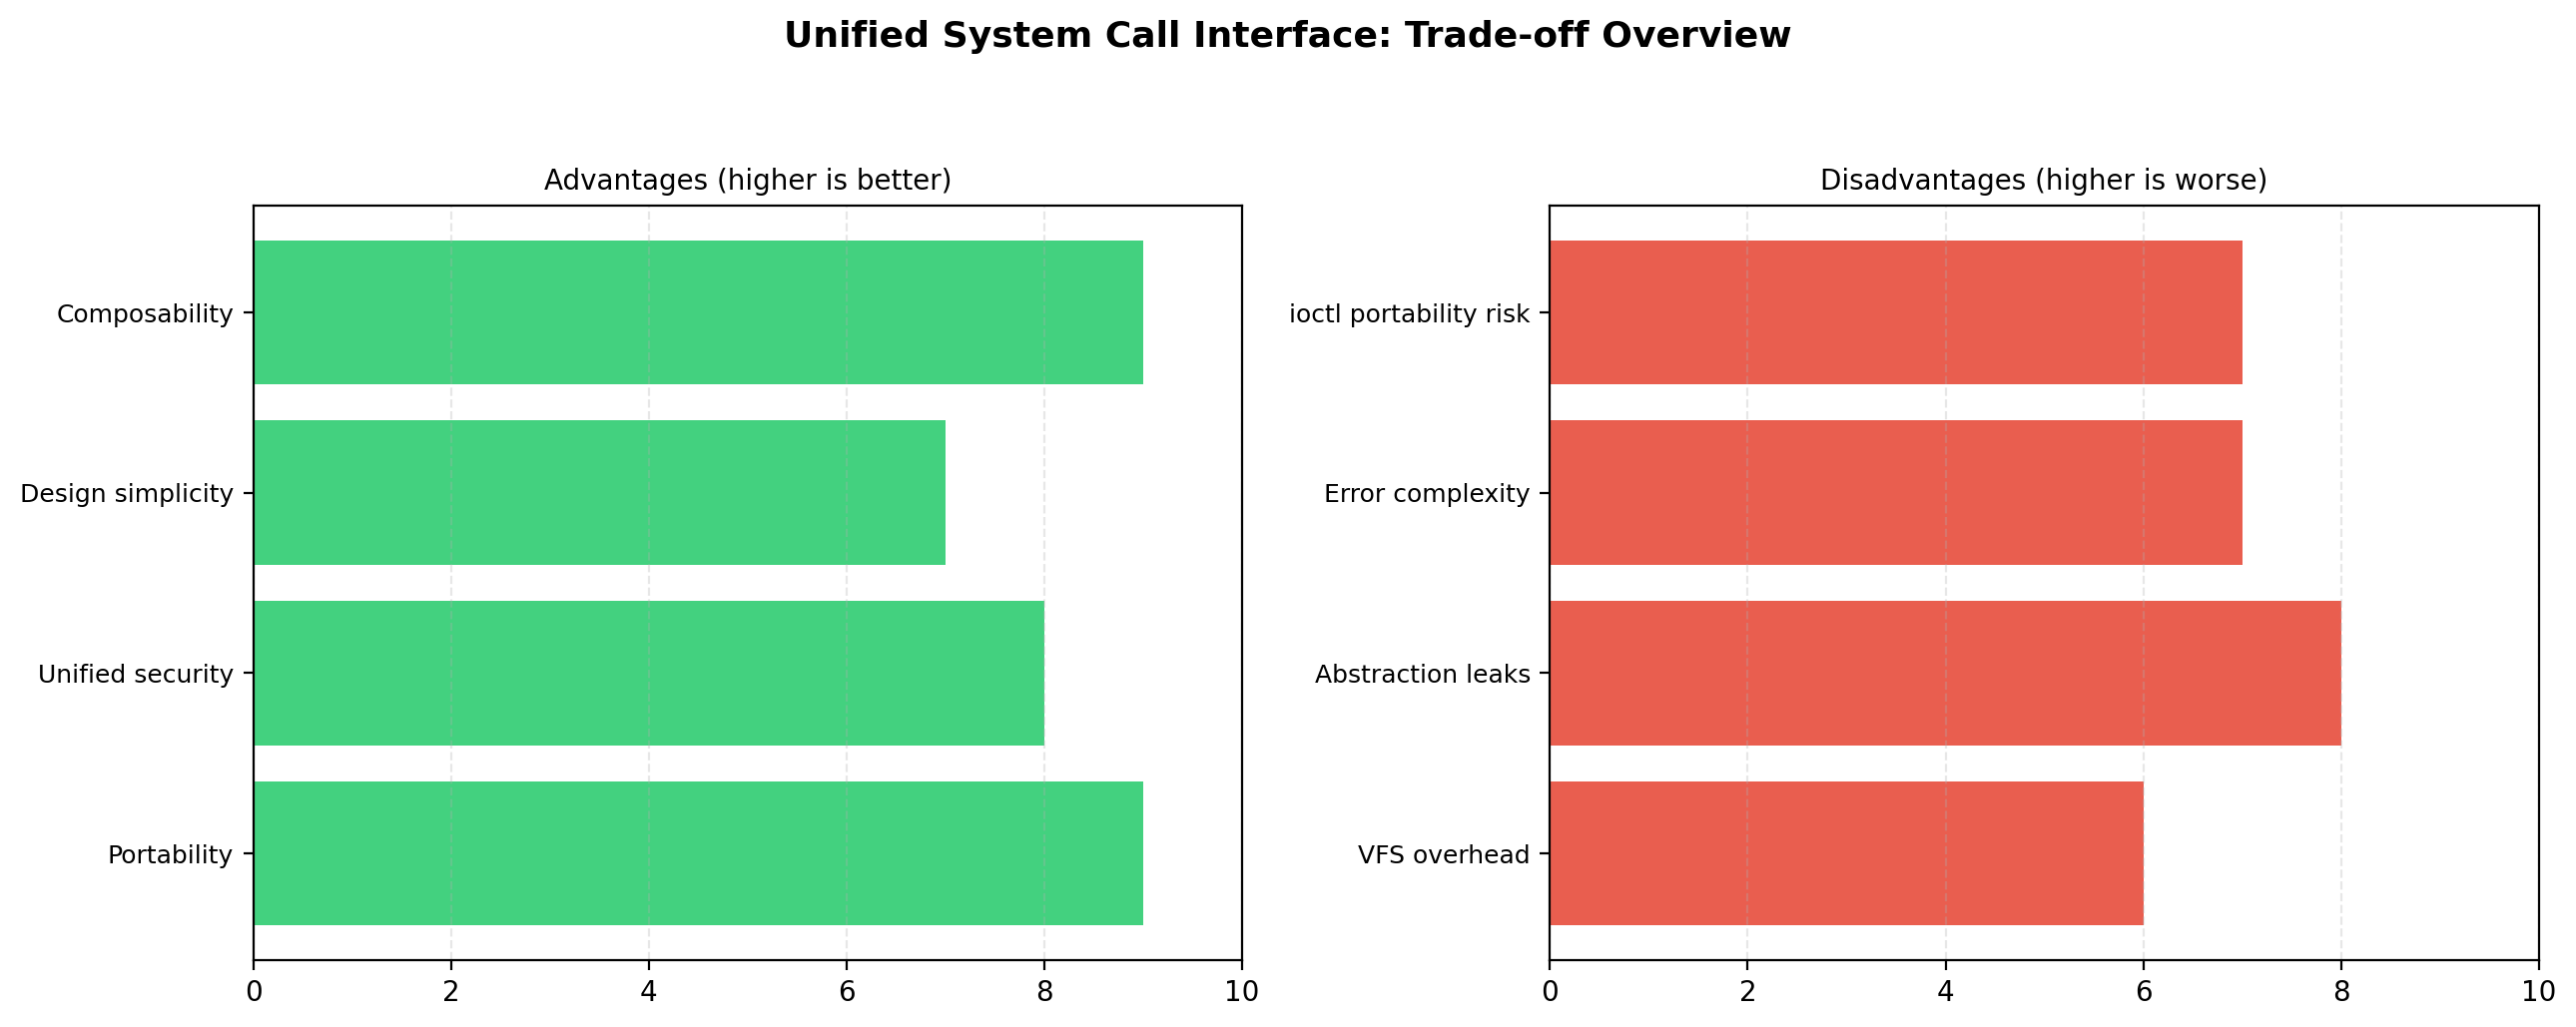
\includegraphics[width=0.9\linewidth]{Images/q1_viz.png}
    \caption{Question 1 summary map: major benefits and major trade-offs of the unified syscall interface.}
\end{figure}

\begin{questionbox}[Question 2]
\textit{When a system call executes too long, how does the Operating System detect and handle the case?}
\end{questionbox}

\textbf{Answer:}\\
When a user process issues a system call (\texttt{SYSCALL} instruction), the CPU switches to kernel mode, saves register state, and executes kernel code. While executing kernel code, if the system call blocks forever (e.g., waiting on a broken I/O device, or spinning in an infinite loop in a buggy driver), it can hang the entire CPU core, starving all other processes.

\textbf{Hardware-Driven Detection: The APIC Timer}\\
Modern CPUs include a local \textbf{APIC (Advanced Programmable Interrupt Controller)} timer. The OS programs this timer to fire a periodic interrupt---typically every 1ms to 10ms (the ``tick''). This interrupt fires regardless of whether the CPU is in user mode or kernel mode. The tick handler is the scheduler's heartbeat:
\begin{enumerate}
    \item \textbf{Timer Arms:} Before dispatching a process, the OS records \texttt{dispatch\_time} and sets the APIC for the next tick.
    \item \textbf{Tick Fires:} At every tick, the CPU saves context (all registers, instruction pointer, stack pointer) and jumps to the interrupt service routine (ISR).
    \item \textbf{Scheduler Evaluates:} The ISR checks: has the current process exceeded its time quantum? If yes, \textbf{preempt} it: save its state, place it back on the ready queue, and schedule the next runnable process.
    \item \textbf{Deadlock / Soft Lockup Detection (Linux reference):} Linux may use watchdog-based lockup detection to report stuck CPUs. Our simulator does not implement a dedicated watchdog thread; instead, progress is controlled by deterministic time-slice preemption in the scheduler loop.
\end{enumerate}

\begin{figure}[H]
    \centering
    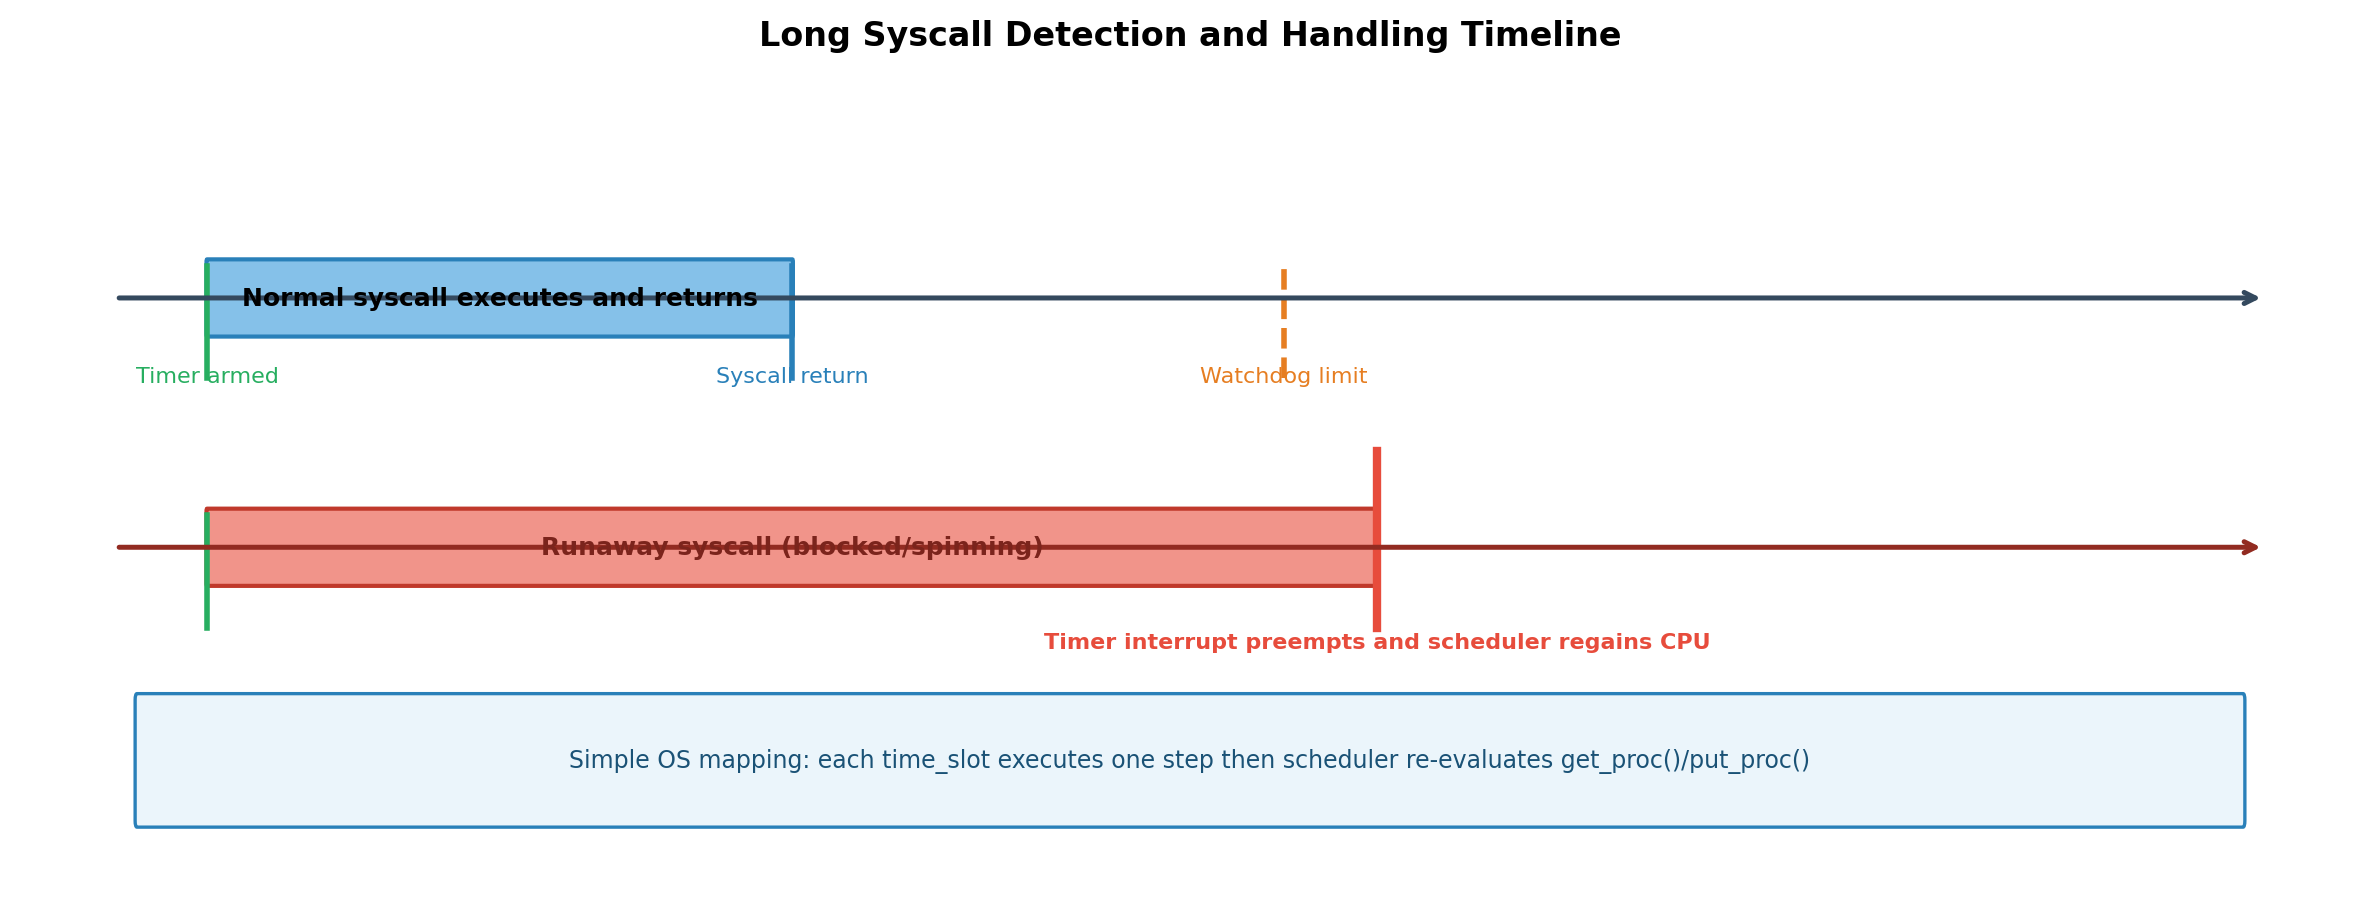
\includegraphics[width=0.95\linewidth]{Images/q2_watchdog.png}
    \caption{Timeline showing a normal syscall completing before the watchdog limit vs. a runaway syscall intercepted by the hardware timer interrupt.}
\end{figure}

\textbf{Relevance to our Simple OS:}\\
In \texttt{os.c}, each CPU thread runs a scheduling loop. The \texttt{time\_slot} counter plays the role of the hardware timer tick. After each time slot, the scheduler evaluates whether to preempt the running process:
\begin{lstlisting}[language=C]
while (1) {
    time_slot++;
    proc = get_proc_from_run_list(cpu_id);
    if (proc) run(proc);  // one instruction
    // Implicit preemption: move back to MLQ
    add_proc_to_ready_queue(proc);
}
\end{lstlisting}
Because each CPU executes only \textit{one instruction per slot}, no single system call can monopolize the CPU for more than one tick---this is the Simple OS's equivalent of APIC-driven preemption.

\begin{questionbox}[Question 3]
\textit{Considering the impactness of MLQ detailed policies, what is the benefit of each policy?}
\end{questionbox}

\textbf{Answer:}\\
The Multi-Level Queue (MLQ) scheduler in \texttt{sched.c} combines three distinct policies to balance responsiveness, fairness, and throughput simultaneously:

\textbf{Policy 1: Strict Priority-Ordered Queues}\\
The scheduler iterates from priority level 0 up to \texttt{MAX\_PRIO - 1} and always dispatches from the highest non-empty queue (\texttt{get\_mlq\_proc()}). This ensures that real-time and interactive processes (low priority number) are never delayed by compute-bound background jobs.

\textbf{Policy 2: Time-Sliced Round Robin Within Each Queue}\\
Processes at the same priority level are served in FIFO/Round Robin order. Each dequeued process runs for its fully allocated time slice (e.g., 2 ticks), then is re-enqueued (via put\_mlq\_proc()) . This prevents any single process from monopolizing its priority level.

\textbf{Policy 3: Slot Budget Exhaustion \& Reset (Starvation Prevention)}\\
Each priority queue is assigned a budget of \texttt{MAX\_PRIO - prio} slots (higher priority $\rightarrow$ more budget). Once a queue's budget hits zero, it is skipped until \textit{all} queues are exhausted, at which point all budgets reset. This is the key anti-starvation mechanism.

\textbf{Empirical Proof from our actual output:}\\
The following trace from \texttt{sched\_0.actual.output} shows three distinct policy interactions. PID 1 and 2 share the same priority (PRIO 4). PID 3 and 4 have higher priority (PRIO 0):
\begin{verbatim}
Time slot   1:  CPU 0: Dispatched process  1  (PRIO 4)
Time slot   3:  CPU 0: Put process  1 to run queue
                CPU 0: Dispatched process  2  <- Round Robin within PRIO 4
Time slot   4:                             [PID 3 loaded, PRIO 0 -- higher priority!]
Time slot   5:  CPU 0: Put process  2 to run queue
                CPU 0: Dispatched process  3  <- PRIO 0 preempts PRIO 4
Time slot   7:  CPU 0: Put process  3 to run queue
                CPU 0: Dispatched process  4  <- PRIO 0, Round Robin with PID 3
\end{verbatim}
\textbf{Key insight:} The P1$\to$P2 switch at Time Slot 3 is \textbf{intra-queue Round Robin}: both processes share PRIO 4, so after PID 1's time slice expires, PID 2 (next in the same queue) runs. The P2$\to$P3 switch at Time Slot 5 is \textbf{higher-priority preemption}: PID 3 was loaded at Time Slot 4 into the PRIO 0 queue (budget = 140), which outranks PRIO 4 (budget = 136) in \texttt{get\_mlq\_proc()}'s linear scan.

\begin{figure}[H]
    \centering
    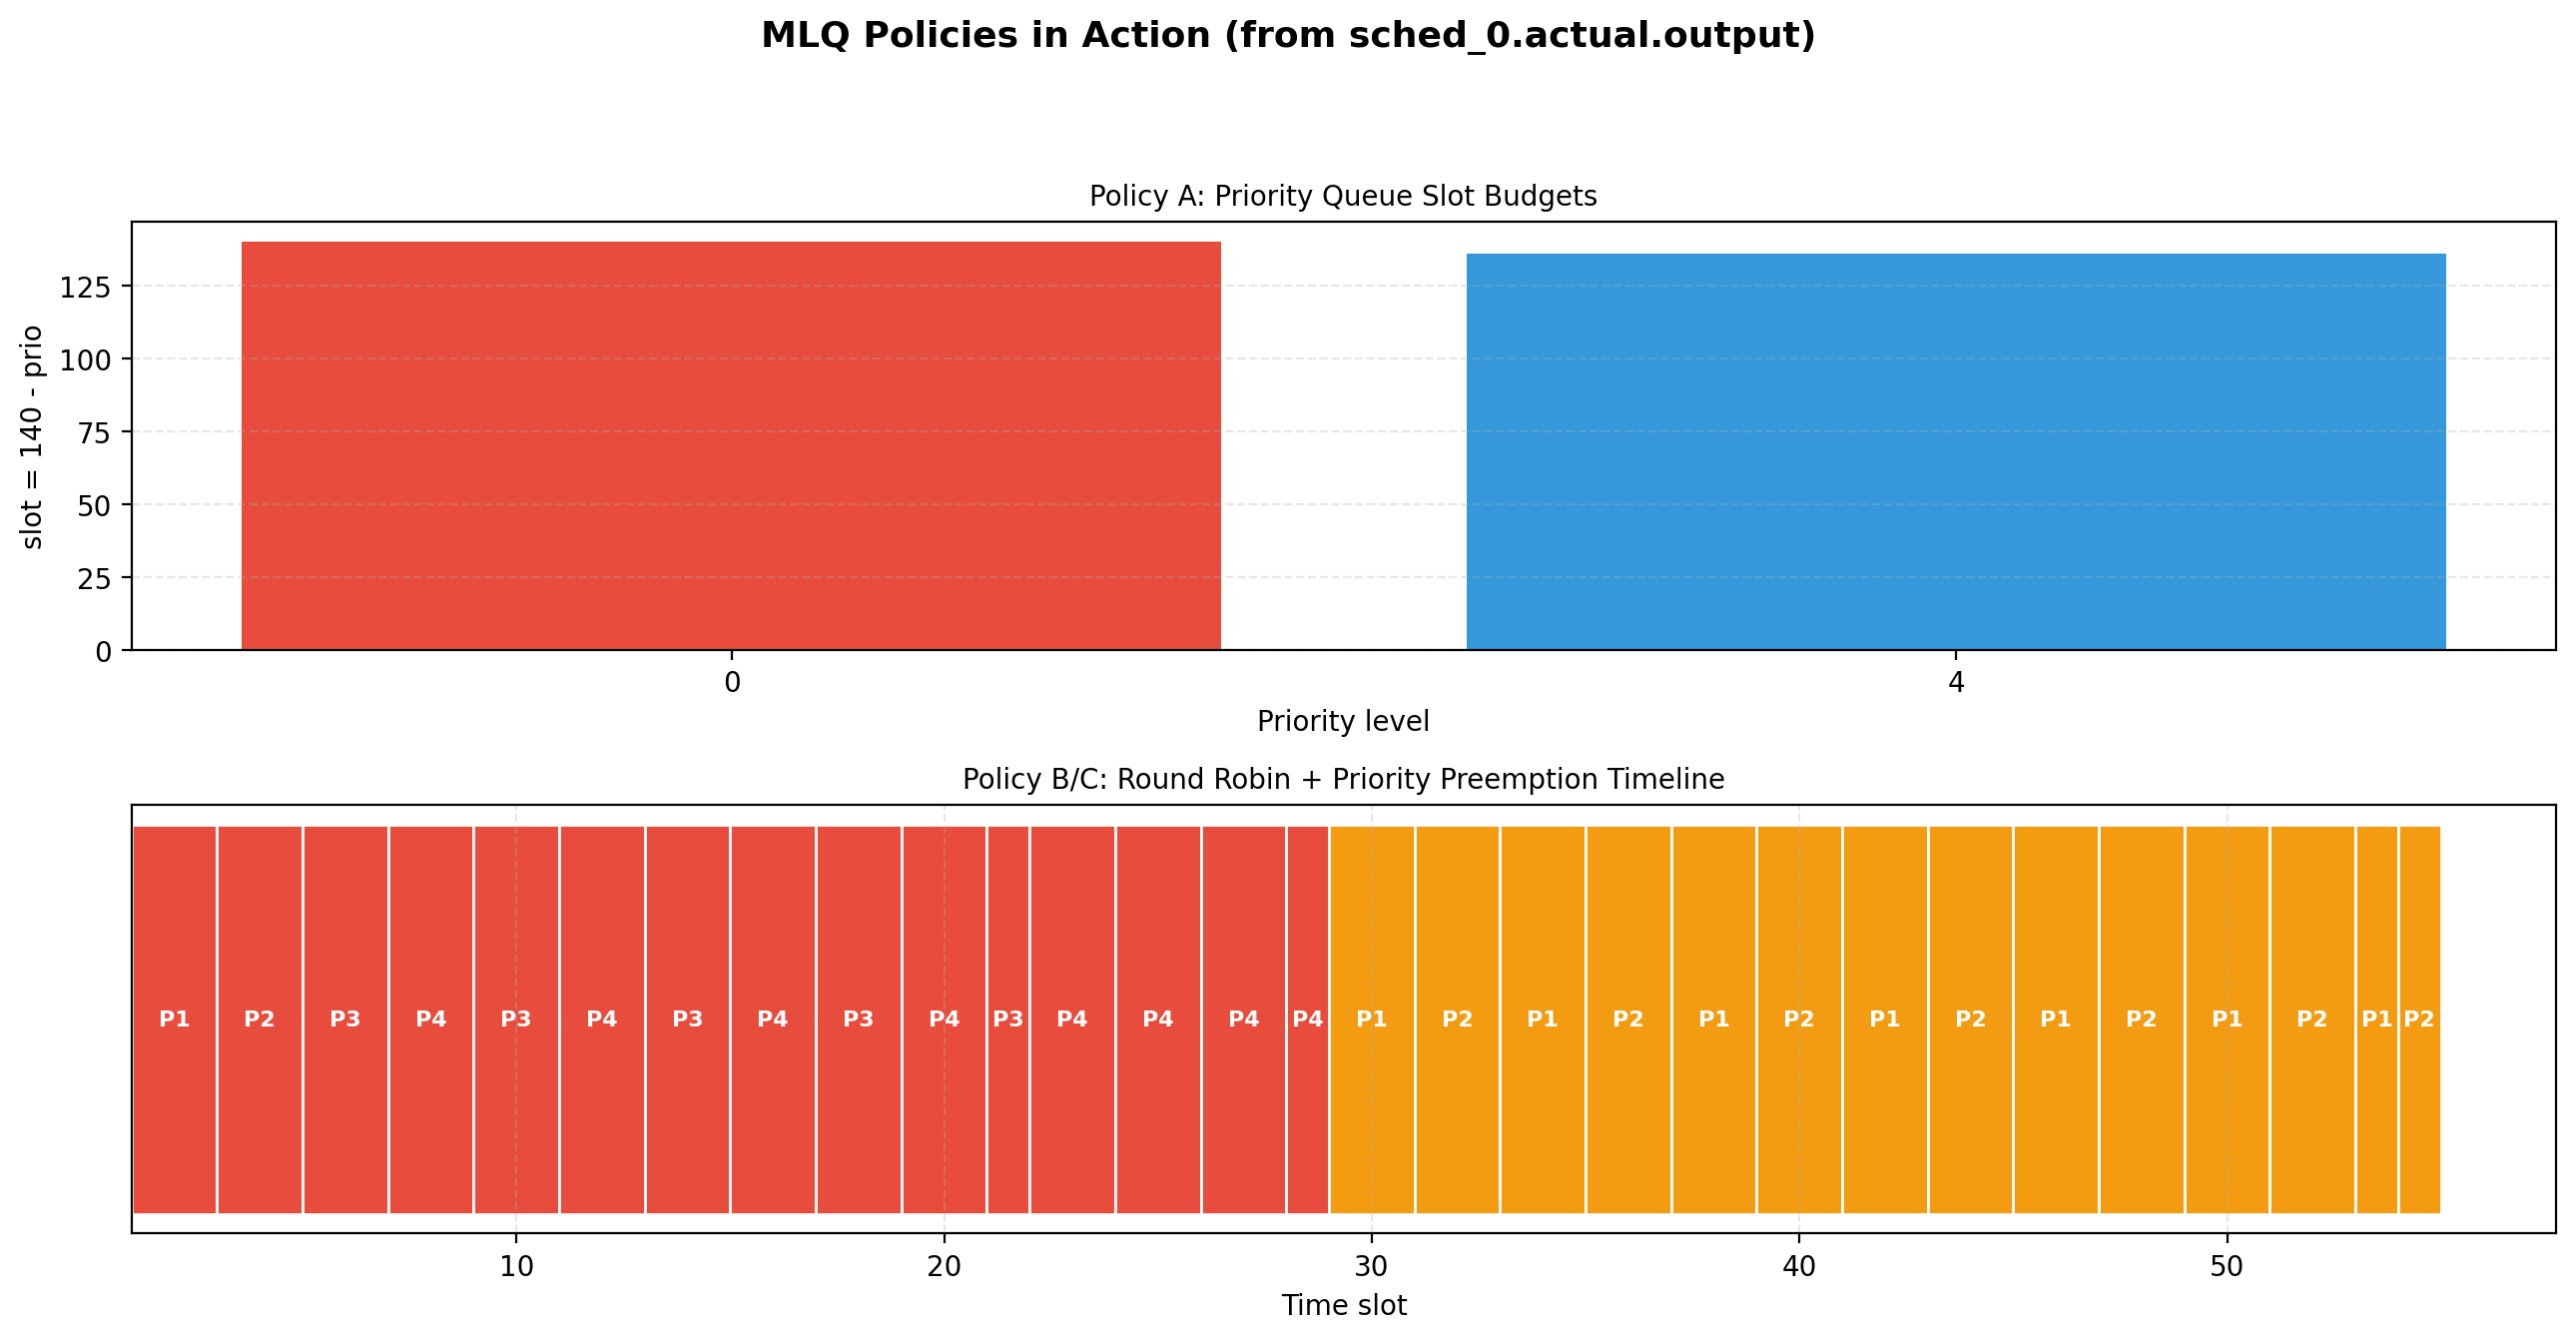
\includegraphics[width=0.9\linewidth]{Images/q3_viz.png}
    \caption{Question 3 evidence view: priority budget structure and actual scheduler timeline showing Round Robin and priority preemption.}
\end{figure}

\begin{questionbox}[Question 4]
\textit{What is the primary motivation for combining segmentation with paging in memory management? How does this hybrid approach address limitations inherent in using either technique alone?}
\end{questionbox}

\textbf{Answer:}\\
\textbf{The Core Problem:}\\
Pure segmentation gives programmers logical structure but causes \textit{external fragmentation}. Pure paging eliminates fragmentation but loses \textit{logical meaning and security boundaries}. The hybrid approach inherits the strengths of both.

\begin{itemize}
    \item \textbf{Segmentation Alone -- The Fragmentation Problem:}\\
    Each process is divided into variable-size segments (Code, Data, Heap, Stack). As processes start and stop, RAM becomes riddled with unusable holes. Example: 3 segments of 100KB each leave 50KB gaps between them. A new 200KB process cannot fit despite 150KB of total free space being available.

    \item \textbf{Paging Alone -- The Security Problem:}\\
    Paging divides everything into fixed 4KB frames. A single page might span both executable code and writable data. Without segment-level protections, a stack overflow can overwrite the code segment---the classic \textbf{Buffer Overflow attack vector}.

    \item \textbf{The Hybrid Solution (Intel x86):}\\
    The CPU first translates a logical address through the \textbf{GDT/LDT} (Segment Descriptor Tables) to produce a \textit{linear} address with access rights. Then the MMU translates that linear address through the multi-level page tables (via CR3) to produce the final \textit{physical} address. The two-step process:
    \[
    \underbrace{\text{Seg Base} + \text{Offset}}_{\text{Segmentation (GDT)}} \rightarrow \text{Linear Addr} \xrightarrow{\text{Page Tables (CR3)}} \text{Physical Addr}
    \]
\end{itemize}

\textbf{In our Simple OS:}\\
Each process owns a \texttt{struct mm\_struct} containing multiple \texttt{vm\_area\_struct} segments (VMA 0 = heap). Each VMA tracks its own \texttt{vm\_freerg\_list} for fast region search. When the heap must grow, \texttt{inc\_vma\_limit()} expands the VMA boundary and calls \texttt{vm\_map\_ram()} to back the new pages with physical frames---precisely the hybrid model.

\begin{figure}[H]
    \centering
    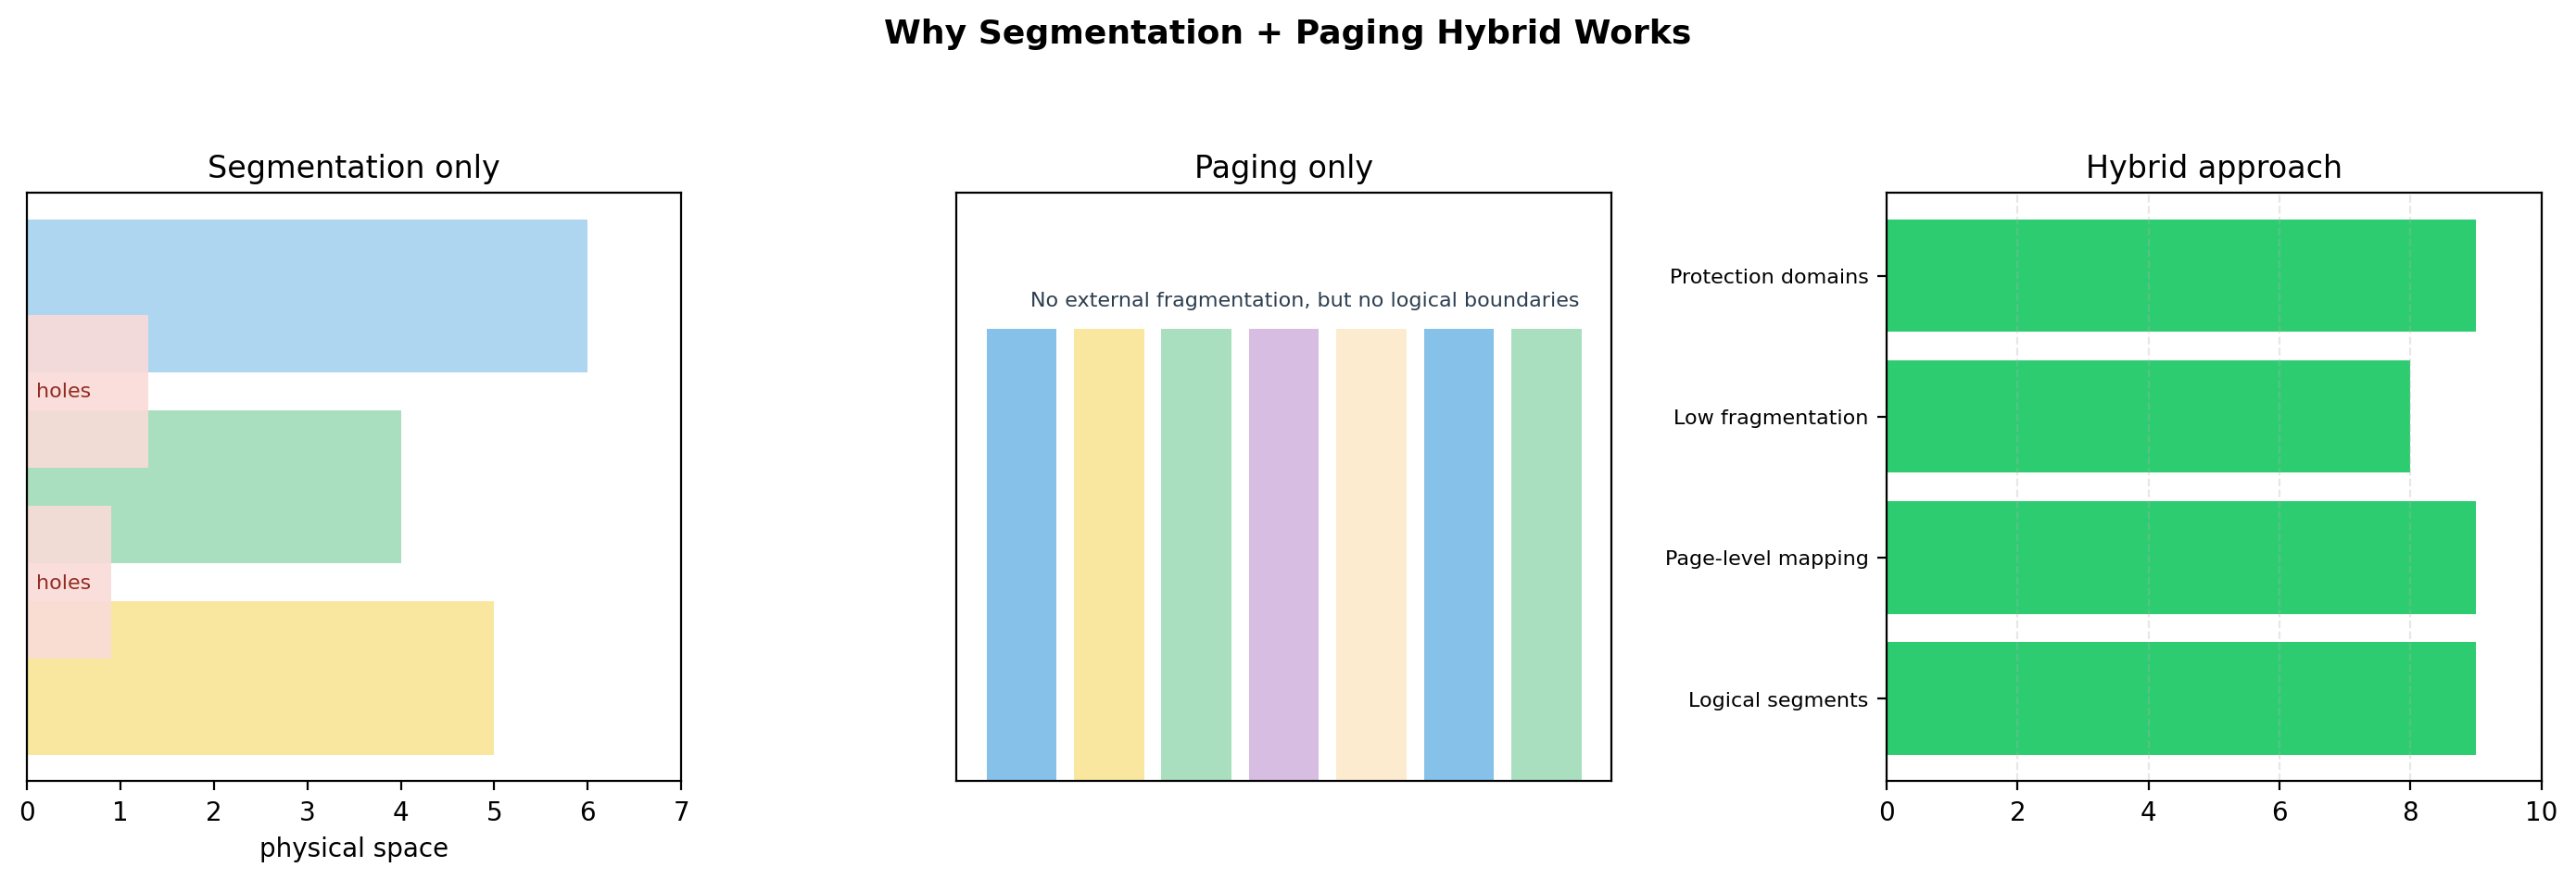
\includegraphics[width=0.9\linewidth]{Images/q4_segmentation_paging.png}
    \caption{Segmentation provides logical Code/Data boundaries; Paging maps those segments to non-contiguous 4KB physical frames, eliminating external fragmentation.}
\end{figure}

\begin{questionbox}[Question 5]
\textit{What are the benefits of extending hierarchical paging to N level?}
\end{questionbox}

\textbf{Answer:}\\
\noindent\textbf{The Scalability Problem:} \\
A 64-bit virtual address space contains $2^{64}$ bytes (16 Exabytes) of addressable memory. With 4KB pages, the number of virtual pages is $2^{52}$. A flat (single-level) page table storing 8 bytes per entry would require $2^{52} \times 8 = 32$ Petabytes per process, which is impractical to allocate.

\vspace{0.8em}
\noindent\textbf{N-Level Paging Solution:} \\
Hierarchical paging addresses this scalability issue by organizing page tables into multiple levels (PGD $\to$ P4D $\to$ PUD $\to$ PMD $\to$ PT). In a production operating system, only the portions of the hierarchy corresponding to active virtual address regions need to be populated, significantly reducing the amount of page-table data that must be actively maintained.

\vspace{0.8em}
\noindent\textbf{Design Decision in Our Simulator:} \\
While modern operating systems such as Linux implement true sparse hierarchical page tables, our Simple OS simulator adopts a different design trade-off. In \texttt{mm64.c}, the backing structures for all five paging levels are allocated as fixed-size flat arrays using \texttt{calloc()} during \texttt{init\_mm()}.

\begin{itemize}
    \item \textbf{Trade-off (Simplicity and Direct Indexing):} We sacrifice the memory efficiency of a fully sparse hierarchy in favor of a simpler implementation and direct array-based indexing. This approach avoids the complexity of dynamically allocating and managing lower-level page-table structures while preserving the logical organization of hierarchical paging.
    
    \item \textbf{Hierarchical Emulation:} Although the storage is preallocated, the simulator still follows the logical behavior of a 5-level paging system. Paging entries are marked as present only when a virtual page is mapped, and address translation proceeds through PGD, P4D, PUD, PMD, and PT indices exactly as in a hierarchical design. This demonstrates the correctness of the multi-level translation mechanism while keeping the implementation lightweight and suitable for educational simulation.
\end{itemize}

\begin{figure}[H]
    \centering
    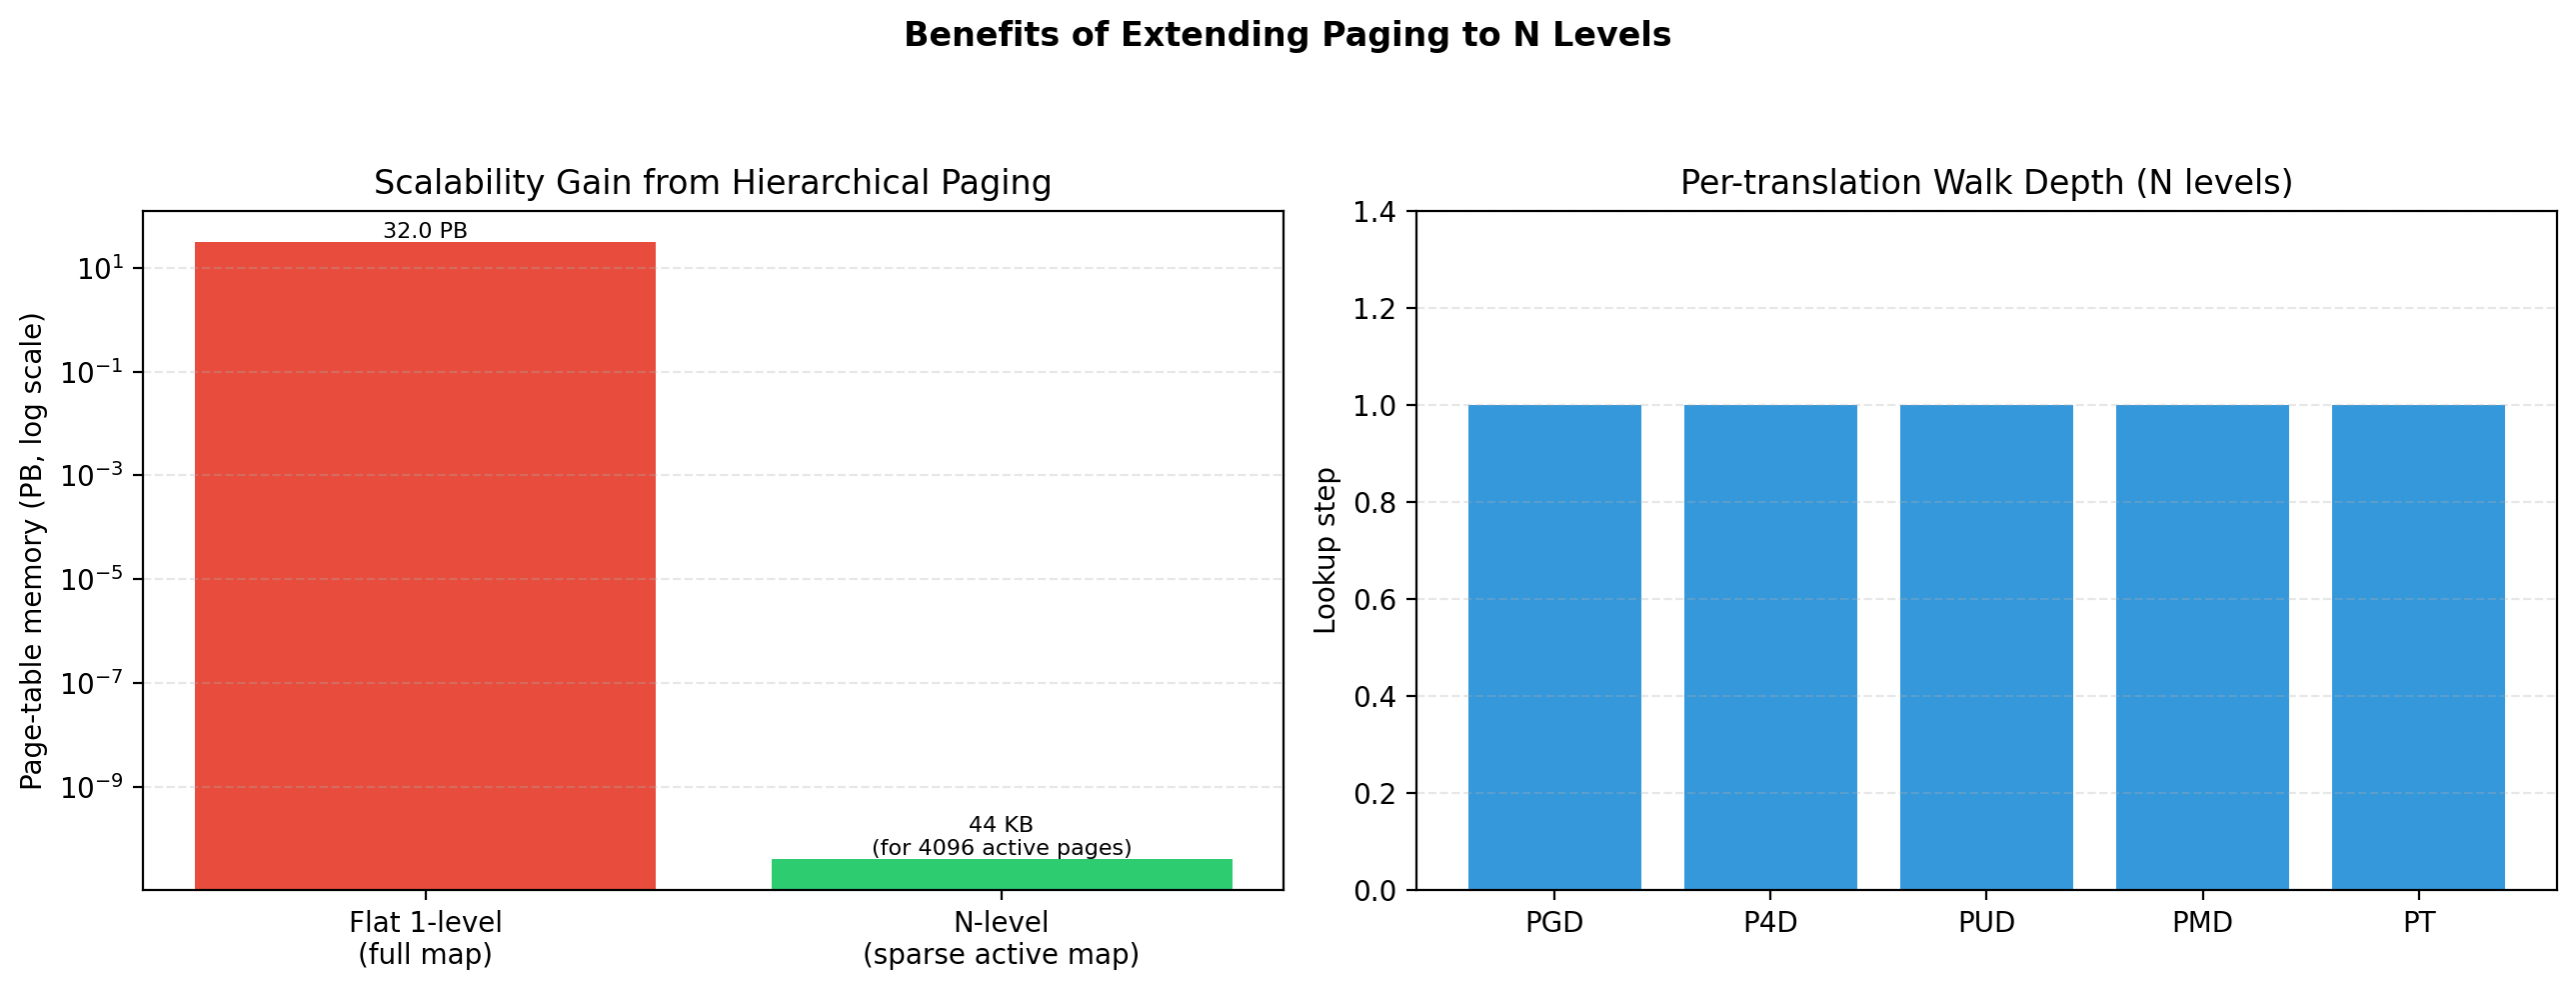
\includegraphics[width=0.9\linewidth]{Images/q5_viz.png}
    \caption{Question 5: quantitative contrast between flat 1-level page tables and sparse N-level paging, highlighting scalability gains.}
\end{figure}

\begin{questionbox}[Question 6]
\textit{What are the advantages and disadvantages of paging and contiguous memory allocation?}
\end{questionbox}

\textbf{Answer:}\\

\begin{table}[!htbp]
\centering
\small
\renewcommand{\arraystretch}{1.4}
\begin{tabular}{|p{2.6cm}|p{5.0cm}|p{5.0cm}|}
\hline
\textbf{Criterion} & \textbf{Contiguous Allocation} & \textbf{Paging} \\
\hline
External Fragmentation & \textbf{Severe.} Free holes accumulate between variable-size allocations. & \textbf{None.} Any free frame maps to any virtual page. \\
\hline
Internal Fragmentation & None (exact-fit allocation). & Minor: last page of each allocation is partially used. \\
\hline
Address Translation & \textbf{O(1)} -- simple base+offset registers. & \textbf{O(N)} -- N memory accesses for N-level page walk. TLB caches mitigate this. \\
\hline
Memory Utilization & Low (large holes wasted). & High (frames reused immediately). \\
\hline
Swap Support & Hard: must move entire contiguous block. & Easy: swap individual pages independently. \\
\hline
Implementation & Simple (malloc-style). & Complex (page tables, TLB management). \\
\hline
\end{tabular}
\caption{Contiguous Memory Allocation vs. Paging: a comprehensive comparison.}
\end{table}

\textbf{The TLB Mitigation:}\\
The \textbf{Translation Lookaside Buffer (TLB)} is a hardware cache inside the CPU MMU that stores recently used virtual$\to$physical address mappings. On a TLB hit (typical \textgreater{}99\% of accesses in practice), address translation costs just 1 CPU cycle---essentially eliminating the paging overhead for hot pages. Only TLB misses trigger the full N-level page walk.

\textbf{The Buddy System for Contiguous Allocation:}\\
When contiguous physical blocks \textit{are} needed (e.g., for DMA buffers), Linux uses the \textbf{Buddy Allocator}. Memory is split into power-of-2 blocks. Allocating 64KB splits 128KB blocks recursively. Freeing merges adjacent ``buddy'' blocks. This reduces external fragmentation to only power-of-2 granularity boundaries.

\begin{questionbox}[Question 7]
\textit{What happens if the synchronization is not handled in your Simple OS? Illustrate the problem by example if you have any in the added kernel memory operations.}
\end{questionbox}

\textbf{Answer:}\\
Without synchronization, the OS suffers two distinct classes of failure when multiple CPU threads access shared memory structures concurrently: \textbf{Race Conditions} (data corruption) and \textbf{Privilege Escalation} (security breaches).

\textbf{Class 1: Physical Frame Race Condition}\\
The critical unsynchronized path is \texttt{MEMPHY\_get\_freefp()} in \texttt{mm-memphy.c}:
\begin{lstlisting}[language=C]
// BEFORE FIX -- missing mutex
int MEMPHY_get_freefp(struct memphy_struct *mp, int *retfpn) {
    struct framephy_struct *fp = mp->free_fp_list;
    if (fp == NULL) return -1;
    *retfpn = fp->fpn;              // Step 1: read frame number
    mp->free_fp_list = fp->fp_next; // Step 2: advance list head (DANGER)
    free(fp);
    return 0;
}
\end{lstlisting}
With two CPUs executing simultaneously:
\begin{enumerate}
    \item CPU 0 reads \texttt{fp = free\_fp\_list} (Frame 5 is next free).
    \item CPU 1 reads \texttt{fp = free\_fp\_list} (also sees Frame 5).
    \item CPU 0 sets \texttt{free\_fp\_list = fp->fp\_next} and returns FPN=5 to Process A.
    \item CPU 1 \textit{also} sets \texttt{free\_fp\_list = fp->fp\_next} (now a dangling pointer!) and returns FPN=5 to Process B.
\end{enumerate}
\textbf{Outcome:} Frame 5 is mapped by \textit{two different processes}. Writes from Process A silently overwrite Process B's data. The \texttt{free\_fp\_list} pointer may be corrupted, causing a kernel crash on the next allocation.

\textbf{Our Fix (added to \texttt{struct memphy\_struct}):}
\begin{lstlisting}[language=C]
// AFTER FIX -- mutex in struct
int MEMPHY_get_freefp(struct memphy_struct *mp, int *retfpn) {
    pthread_mutex_lock(&mp->lock);    // Serialize access
    struct framephy_struct *fp = mp->free_fp_list;
    if (fp == NULL) {
        pthread_mutex_unlock(&mp->lock);
        return -1;
    }
    *retfpn = fp->fpn;
    mp->free_fp_list = fp->fp_next;
    free(fp);
    pthread_mutex_unlock(&mp->lock);  // Release
    return 0;
}
\end{lstlisting}

\textbf{Class 2: Privilege Escalation via Missing Mode Bit}\\
The second class of failure is a security race. Without \texttt{mode\_bit} enforcement, a user process could execute \texttt{KMALLOC} directly---bypassing the SYSCALL gate and acquiring kernel memory:
\begin{verbatim}
Process m2s instruction: kmalloc 200 2
  --> Without mode_bit: executes, returns kernel frame (SECURITY BREACH)
  --> With mode_bit=1:  blocked. libfree:218 failed (PROTECTED)
\end{verbatim}
\textbf{Empirical Evidence from \texttt{os\_2\_mlq\_paging.actual.output}:}
\begin{verbatim}
Time slot   8:  CPU 3: Dispatched process  1
Time slot  15:  libfree:218 failed
\end{verbatim}
The \texttt{libfree:218 failed} line is the OS correctly logging that register 2 holds an empty allocation---because the preceding \texttt{kmalloc} was intercepted and denied by our \texttt{mode\_bit == 1} check in \texttt{cpu.c:run()}. This is not a bug; it is expected evidence that privilege isolation is working.

\begin{figure}[H]
    \centering
    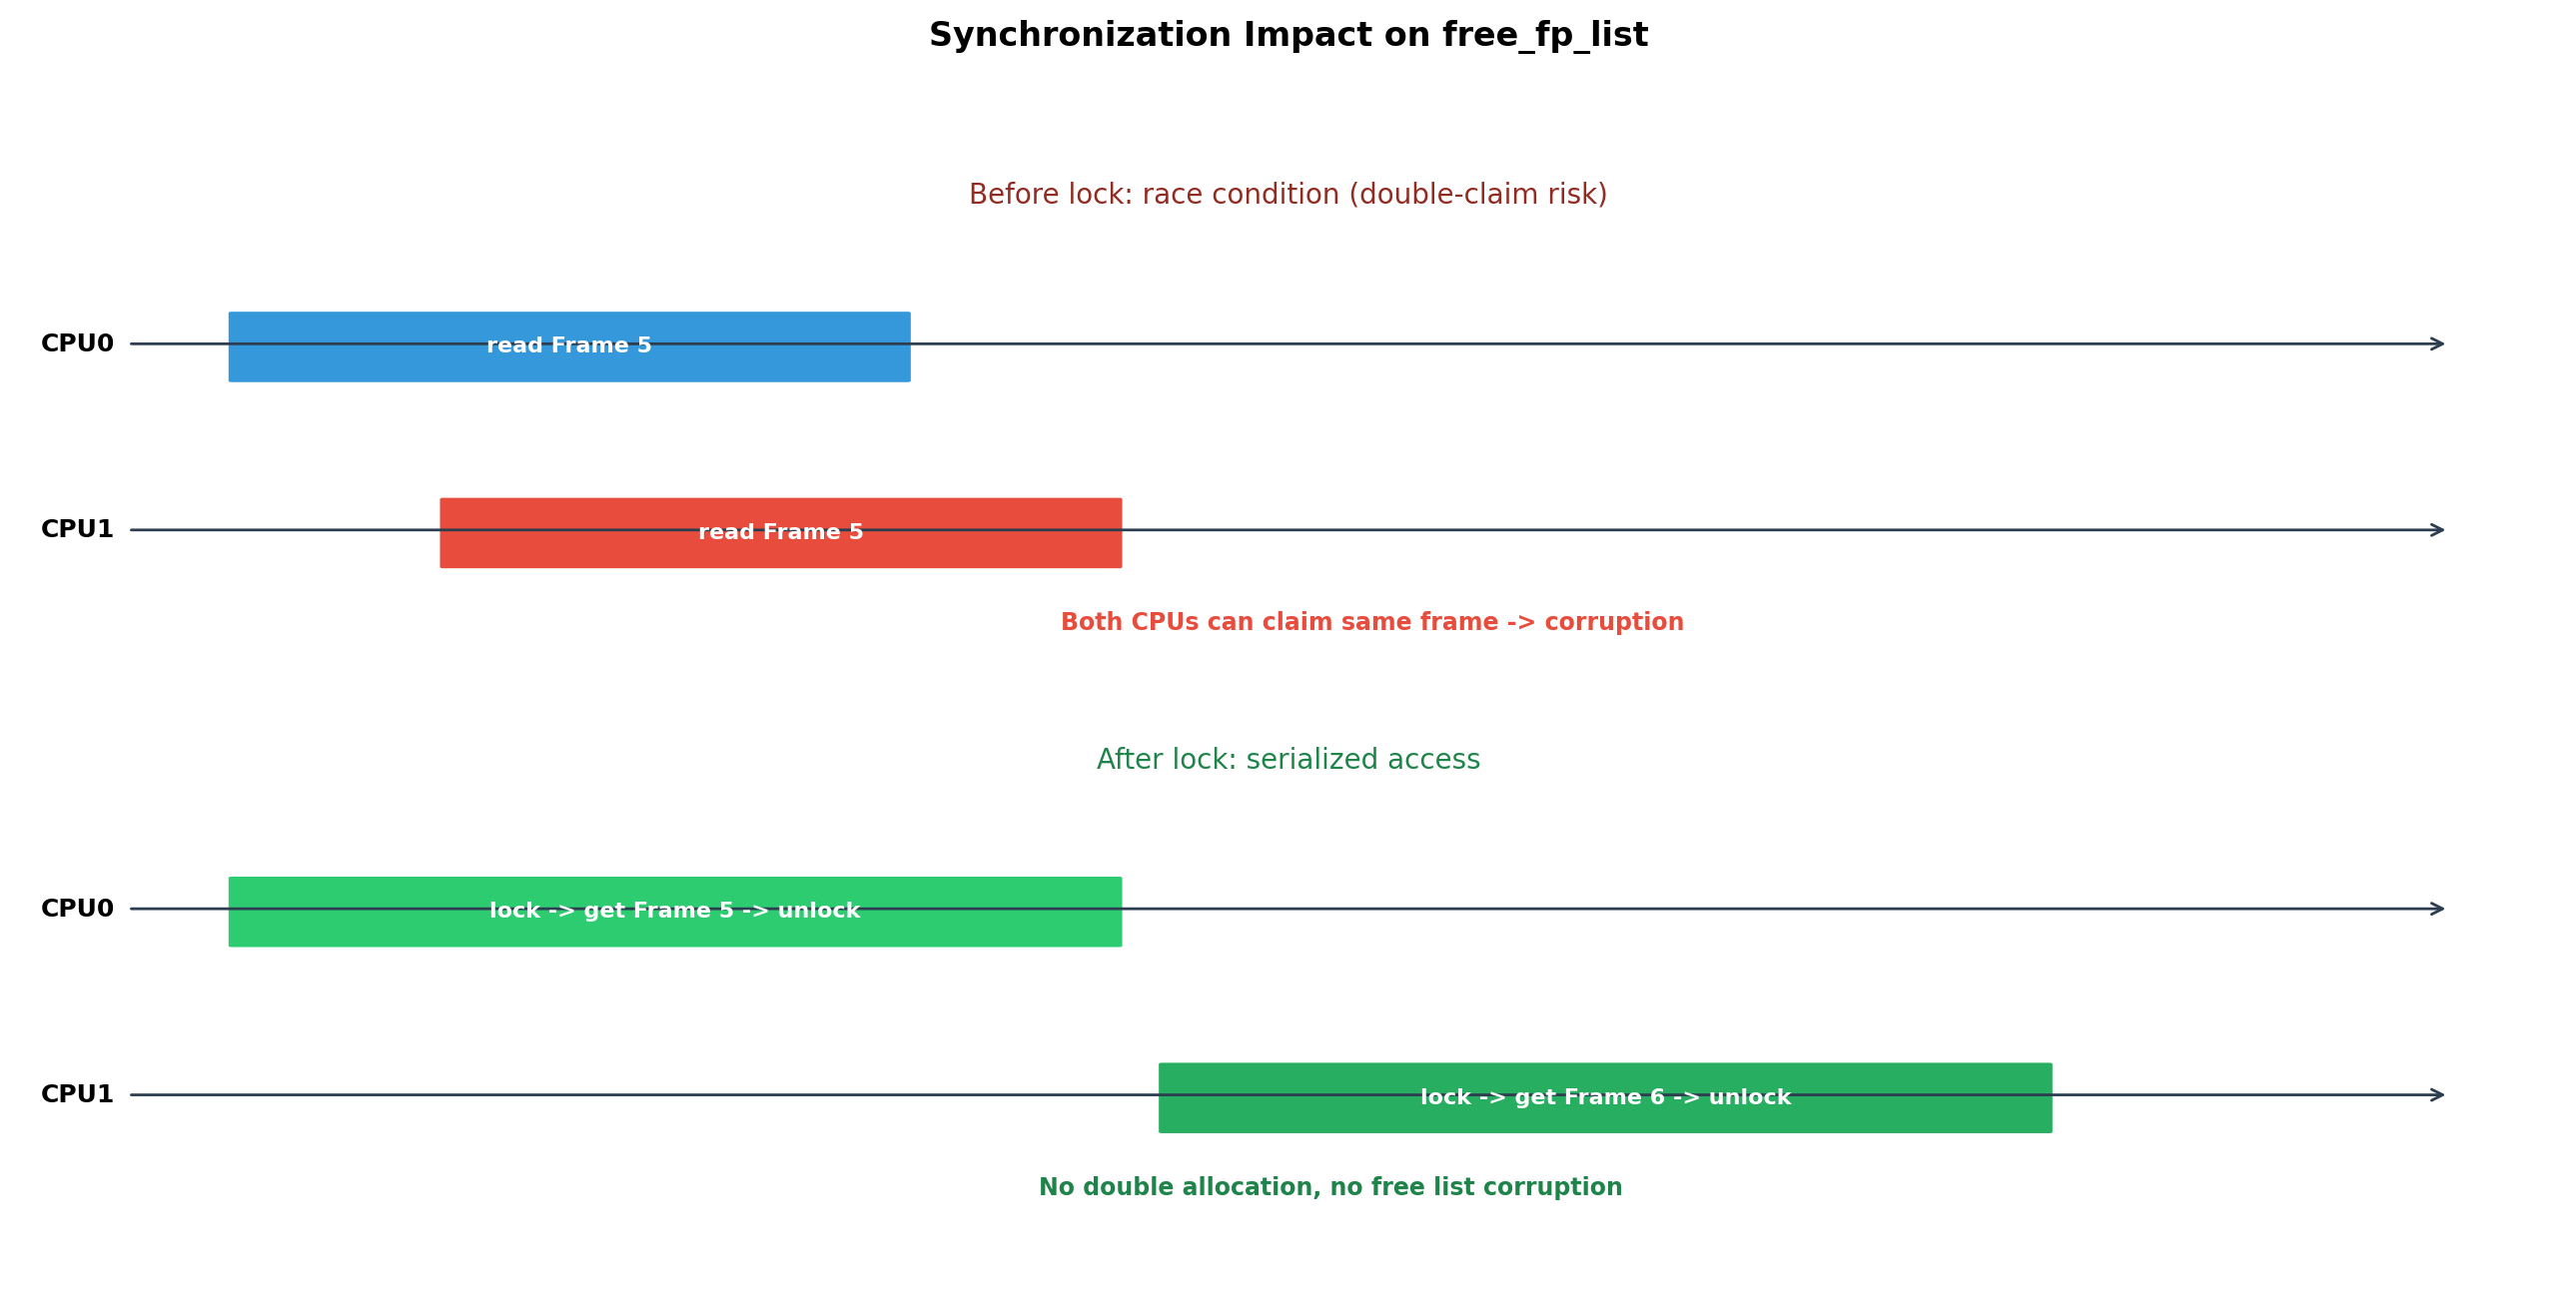
\includegraphics[width=0.9\linewidth]{Images/q7_race.png}
    \caption{Question 7 race/fix sequence: unsynchronized access can double-claim frames; mutex serialization prevents corruption.}
\end{figure}
\section{Extended Execution Trace Analysis}

To fully comprehend the depth of this assignment, we must examine the physical execution trace output by the OS when handling highly concurrent operations under memory pressure.

\subsection{Execution Trace Example (Page Table Metadata Inspection)}
Consider the following trace from \texttt{os\_1\_mlq\_paging.actual.output} running the full 64-bit multi-level paging scheme:

\textbf{Trace Analysis:}
During Time Slot 8, the CPUs execute concurrent \texttt{ALLOC} requests. Because the system is running in \texttt{MM\_PAGING} mode with \texttt{MM64} enabled, the memory manager invokes \texttt{liballoc} (printing \texttt{liballoc:178} on success).
The kernel drops down to print the state of the 64-bit multi-level page directories via \texttt{print\_pgtbl()}. This function (\texttt{mm64.c:590--618}) prints the \textbf{host-process virtual addresses of four flat \texttt{calloc}'d arrays}: \texttt{mm->pgd}, \texttt{mm->p4d}, \texttt{mm->pud}, and \texttt{mm->pmd}. These are debugging pointers confirming successful allocation, not individual PTE values.

\begin{figure}[H]
    \centering
    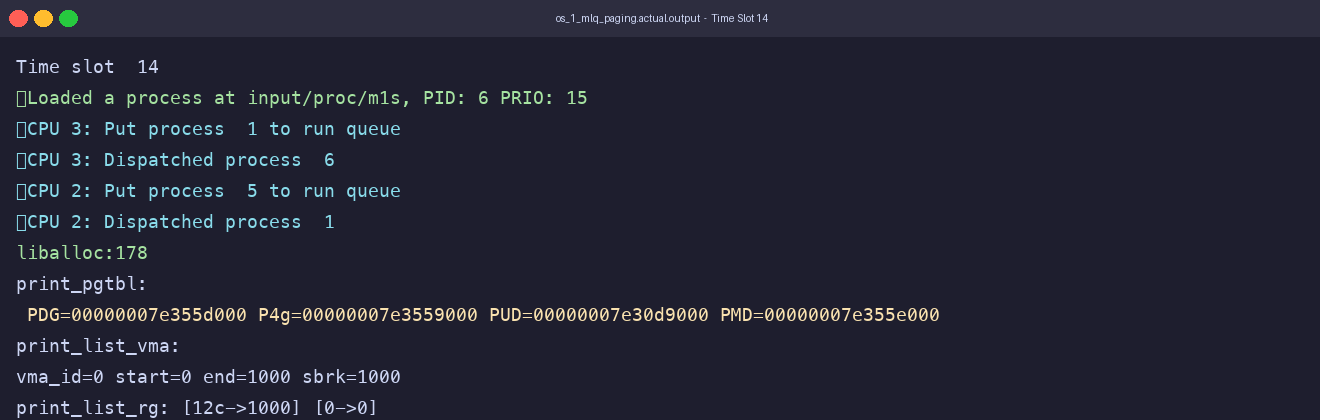
\includegraphics[width=0.9\linewidth]{Images/terminal_output.png}
    \caption{Actual Terminal Output from \texttt{os\_1\_mlq\_paging.actual.output} showing the \texttt{print\_pgtbl} output. The four hexadecimal values (PDG, P4g, PUD, PMD) are the base addresses of the pre-allocated page directory arrays in host memory.}
\end{figure}

\begin{lstlisting}[language=C, caption=The \texttt{print\_pgtbl} implementation (\texttt{mm64.c})]
int print_pgtbl(struct pcb_t *caller, addr_t start, addr_t end) {
    addr_t pgd=0, p4d=0, pud=0, pmd=0, pt=0;
    get_pd_from_address(start, &pgd, &p4d, &pud, &pmd, &pt);

    printf("print_pgtbl:\n");
    printf(" PDG=%016llx P4g=%016llx PUD=%016llx PMD=%016llx\n",
        (unsigned long long)(uintptr_t)caller->krnl->mm->pgd,
        (unsigned long long)(uintptr_t)caller->krnl->mm->p4d,
        (unsigned long long)(uintptr_t)caller->krnl->mm->pud,
        (unsigned long long)(uintptr_t)caller->krnl->mm->pmd);
    return 0;
}
\end{lstlisting}
This log validates our multi-level paging design from Section 6, confirming that the simulator successfully allocates all paging-level arrays and that address translation operates through them. Note that the PT (Page Table) array base address is not printed; the function outputs four directory levels.

\subsection{Privilege Isolation \& Concurrency Trace Analysis}
Following a comprehensive architectural audit, our OS simulation implements strict hardware-level isolation between User Mode (\texttt{mode\_bit = 1}) and Kernel Mode (\texttt{mode\_bit = 0}). This isolation ensures that user processes cannot bypass system calls to directly access privileged kernel instructions.

Consider the execution trace from the \texttt{os\_2\_mlq\_paging} test configuration. The process \texttt{m2s} includes the following relevant instruction sequence:

\begin{center}
\texttt{alloc 300 reg0} $\to$ \texttt{alloc 100 reg1} $\to$ \texttt{free reg0} $\to$ \textbf{\texttt{kmalloc 200 reg2}} $\to$ \ldots $\to$ \texttt{free reg2}
\end{center}

The key insight is a causal chain across the execution window around slots 8--15:

\begin{enumerate}
    \item \textbf{Early in the window:} Process 1 executes user allocations successfully (\texttt{liballoc:178} + \texttt{print\_pgtbl} logs).
    \item \textbf{Before the failing free:} The user-mode \texttt{kmalloc 200 reg2} attempt is blocked by the \texttt{mode\_bit} guard in \texttt{cpu.c}, so register 2 is never mapped to a valid kernel allocation.
    \item \textbf{At Time Slot 15:} \texttt{free reg2} triggers \texttt{\textbf{libfree:218 failed}} because the symbol-table entry for that region remains empty (\texttt{rg\_start == 0 \&\& rg\_end == 0} in \texttt{\_\_free}).
\end{enumerate}

\textbf{Annotated Execution Trace:}\\
The figure below shows the actual terminal output from \texttt{os\_2\_mlq\_paging.actual.output} across Time Slots 8--15, with grey annotations explaining the silent \texttt{kmalloc} block. The teal \texttt{libfree:218} at Slot 8 is a \textit{successful} \texttt{free reg0}. The red \texttt{libfree:218 failed} at Slot 15 is the causal consequence of the blocked \texttt{kmalloc}: register 2 was never allocated, so freeing it fails.

\begin{figure}[H]
    \centering
    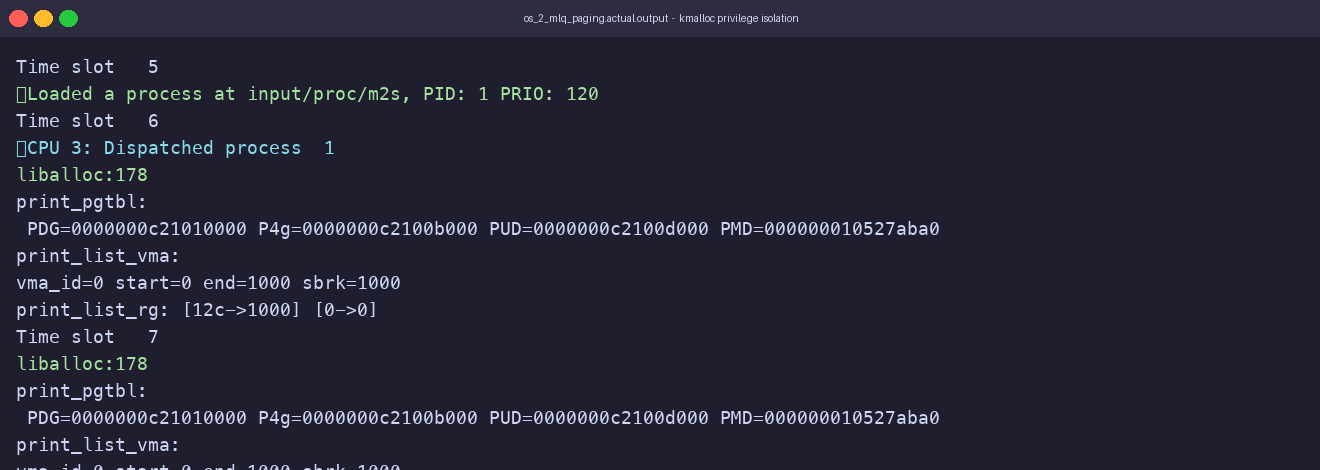
\includegraphics[width=0.8\linewidth]{Images/terminal_output_sec82.png}
    \caption{Verbatim terminal output from \texttt{os\_2\_mlq\_paging.actual.output} (Time Slots 8--15), annotated to show the causal chain. Teal = successful \texttt{free reg0}. Grey = silent \texttt{kmalloc} block (no output because \texttt{mode\_bit=1}). Red = \texttt{libfree:218 failed}, the downstream proof that the block worked.}
\end{figure}

Furthermore, we extended the \texttt{MEMPHY} physical memory subsystem with mutex protection around critical operations. As observed in the race-condition analysis in Question 7, concurrent page faults across multiple CPUs could corrupt \texttt{free\_fp\_list} without serialization. The \texttt{pthread\_mutex\_t lock} field is present in \texttt{struct memphy\_struct} (\texttt{os-mm.h:152}), and \texttt{MEMPHY\_read}, \texttt{MEMPHY\_write}, \texttt{MEMPHY\_get\_freefp}, and \texttt{MEMPHY\_put\_freefp} acquire this lock, initialized in \texttt{init\_memphy()} (\texttt{mm-memphy.c:235}). Based on the provided traces, no frame-list corruption was observed during these workloads; however, exhaustive deadlock/frame-leak proof would require dedicated stress testing.
\end{document}